\chapter[Dark Matter searches with neutrinos from the Sun]{Dark Matter searches\\ with neutrinos from the Sun}\label{chapter:dm_analysis}

\begin{chapquote}{Leo Tolstoy, \textit{Anna Karenina}}
	He stepped down, trying not to look long at her, as if she were the Sun, yet he saw her, like the Sun, even without looking.
\end{chapquote}

%Solar DM capture
The idea of detecting neutrino signals coming from the core of the Sun to probe DM is not new. The main focus of these searches has usually been high-energy neutrinos originated from DM annihilations into heavy particles \cite{Silk1985, Srednicki1986, Hagelin1986, Gaisser1986}. However, recent studies have proposed to look at the low-energy neutrino flux arising from the decay of light mesons at rest in the Sun \cite{Bernal2012, Rott2012, Rott2015, DUNE2021}, previously thought undetectable.

%
In this Chapter, I try to demonstrate the capability of DUNE to constrain different DM scenarios. I use the neutrino fluxes arising from DM annihilations in the core of the Sun to compute the projected limits that DUNE would be able to set on the annihilation rates of DM particles in the Sun and the DM scattering cross sections.

\section{Gravitational capture of DM by the Sun}
\label{sec:dm_analysis_theory}

The Sun and the centre of the Earth are possible sources of DM annihilations, specially interesting because of their proximity. Their gravitational attraction ensures the capture of DM from the local halo through repeated scatterings of DM particles crossing them. Only neutrinos produced from DM annihilations can escape the dense interior of these objects. Therefore, neutrino telescopes are the most useful experimental layouts to pursue DM searches from their cores.

The neutrino flux from DM annihilations inside the Sun depends on the DM capture rate, which is proportional to the DM scattering cross section, and the annihilation rate, which is proportional to the velocity-averaged DM annihilation cross section. The total number of DM particles inside the Sun follows the Boltzmann equation \cite{Bernal2012}:
\begin{equation}\label{2.1}
	\frac{\mathrm{d} N_{DM}}{\mathrm{d} t} = C_{\odot} - A_{\odot} N_{DM}^{2},
\end{equation}
where $C_{\odot}$ and $A_{\odot}$ are the total Sun DM capture and annihilation rates respectively. In this expression I neglected the evaporation term, proportional to $N_{DM}$, which only contribute for $m_{DM}\lesssim 4$ GeV \cite{Busoni2013}. As the current threshold of neutrino telescopes is a few GeV, this region falls below the probed range but can be important in future low-energy projects like DUNE.

This equation has an equilibrium solution:
\begin{equation}\label{2.2}
	N_{DM}^{eq} = \sqrt{\frac{C_{\odot}}{A_{\odot}}},
\end{equation}
which represents the amount of DM inside the Sun if the capture and annihilation have reached equilibrium. As the Sun is approximately $4.6$ Gyr old \cite{Bahcall1995}, it is usually assumed that equilibrium has been achieved. Therefore, the anomalous neutrino flux from the Sun would only depend on the DM scattering cross section, enabling us to set limits on this quantity. If one does not assume equilibrium, some assumptions on the DM annihilation cross section are necessary to extract predictions from neutrino signals.

Here, I am going to consider three possible scenarios for the DM interactions: DM scattering off electrons, spin-dependent (SD) and spin-independent (SI) interactions with nuclei. For these last two, the cross sections will be given in terms of the SD and SI elastic scattering DM cross section off protons (assuming that the DM interactions with protons and neutrons are identical), $\sigma_{p}^{\mathrm{SD}}$ and $\sigma_{p}^{\mathrm{SI}}$, as \cite{Bernal2012,Palomares2017}:
\begin{align}\label{2.3-2.4}
	\sigma_{i}^{\mathrm{SD}} &= \left(\frac{\tilde{\mu}_{A_{i}}}{\tilde{\mu}_{p}}\right)^{2} \frac{4(J_{i}+1)}{3 J_{i}} |\expval{S_{p,i}} + \expval{S_{n,i}}|^{2} \sigma_{p}^{\mathrm{SD}},\\
	\sigma_{i}^{\mathrm{SI}} &= \left(\frac{\tilde{\mu}_{A_{i}}}{\tilde{\mu}_{p}}\right)^{2} A_{i}^{2} \sigma_{p}^{\mathrm{SI}},
\end{align}
where $\tilde{\mu}_{A_{i}}$ is the reduced mass of the DM-nucleus $i$ system, $\tilde{\mu}_{p}$ is the reduced mass of the DM-proton system, $A_{i}$ and $J_{i}$ the mass number and total angular momentum of nucleus $i$, and $\expval{S_{p,i}}$ and $\expval{S_{n,i}}$ the expectation value of the spins of protons and neutrons averaged over all nucleons, respectively (see Ref. \cite{Bednyakov2004} for a review on spin expectation values).

Since the Sun is mainly composed of hydrogen, the capture of DM from the halo is expected to occur mainly through SD scattering. However, since the SI cross section is proportional to the square of the atomic mass, heavy elements can contribute to the capture rate (even though they constitute less than $2\%$ of the mass of the Sun). Heavy elements can also contribute to the SD cross section if the DM also has momentum-dependent interactions \cite{Catena2015}.

DM particles can get captured by the Sun if after repeated scatterings off solar targets their final velocity is lower than the escape velocity of the Sun. In the limit of weak cross sections, this capture rate can be approximately written as \cite{Gould1987}:
\begin{equation}\label{2.5}
	C_{\odot}^{\mathrm{weak}} = \sum_{i} \int_{0}^{R_{\odot}} \mathrm{d}r \ 4\pi r^{2} \int_{0}^{\infty} \mathrm{d}u_{\chi} \ \frac{\rho_{\chi}}{m_{\chi}} \frac{f_{v_{\odot}}(u_{\chi})}{u_{\chi}} \omega(r) \int_{0}^{v_{e}(r)} \mathrm{d}v \ R_{i}^{-}(\omega \rightarrow v) |F_{i}(q)|^{2},
\end{equation}
where the summation extends over all possible solar targets. In this expression, $R_{\odot}$ is the radius of the Sun, $\rho_{\chi}$ is the local DM density, $m_{\chi}$ the mass of the DM particle, $f_{v_{\odot}}(u_{\chi})$ the DM velocity distribution seen from the Sun's reference frame, $R_{i}^{-}(\omega \rightarrow v)$ is the differential rate at which a DM particle with velocity $v$ scatters a solar target of mass $m_{i}$ to end up with a velocity $\omega$ and $|F_{i}(q)|$ is the nuclear form factor of target $i$.

The differential scattering rate takes a rather simple form when considering velocity-independent and isotropic cross sections. In that case, this quantity is given by \cite{Gould1987, Palomares2017}:
\begin{equation}\label{2.6}
	R_{i}^{-}(\omega \rightarrow v) = \frac{2}{\sqrt{\pi}} \frac{\mu_{i,+}^{2}}{\mu_{i}} \frac{v}{\omega} n_{i}(r) \sigma_{i} \left[\chi(- \alpha_{-}, \alpha_{+})+\chi(- \beta_{-}, \beta_{+}) \mathrm{e}^{\mu_{i}(\omega^{2}-v^{2})/u_{i}^{2}(r)}\right],
\end{equation}
where $\mu_{i}$ is the ratio between the DM mass and the mass of target $i$, $\mu_{i,\pm}$ is defined as:
\begin{equation}\label{2.7}
	\mu_{i,\pm} \equiv \frac{\mu_{i} \pm 1}{2},
\end{equation}
$n_{i}(r)$ is the density profile of target $i$ in the solar medium, $u_{i}(r)$ is the most probable velocity of target $i$ given by:
\begin{equation}\label{2.8}
	u_{i}(r) = \sqrt{\frac{2 T_{\odot}(r)}{m_{i}}},
\end{equation}
where $T_{\odot}(r)$ is the temperature of the Sun, the quantities $\alpha_{\pm}$ and $\beta_{\pm}$ are defined as:
\begin{align}\label{2.9-2.10}
	\alpha_{\pm} &\equiv \frac{\mu_{i,+} v \pm \mu_{i,-} \omega}{u_{i}(r)},\\
	\beta_{\pm} &\equiv \frac{\mu_{i,-} v \pm \mu_{i,+} \omega}{u_{i}(r)},
\end{align}
and the function $\chi(a,b)$ is a Gaussian integral of the form:
\begin{equation}\label{2.11}
	\chi(a,b) \equiv \int_{a}^{b} \mathrm{d}x \ \mathrm{e}^{-x^{2}}. 
\end{equation}

\begin{figure}[t]
	\centering
	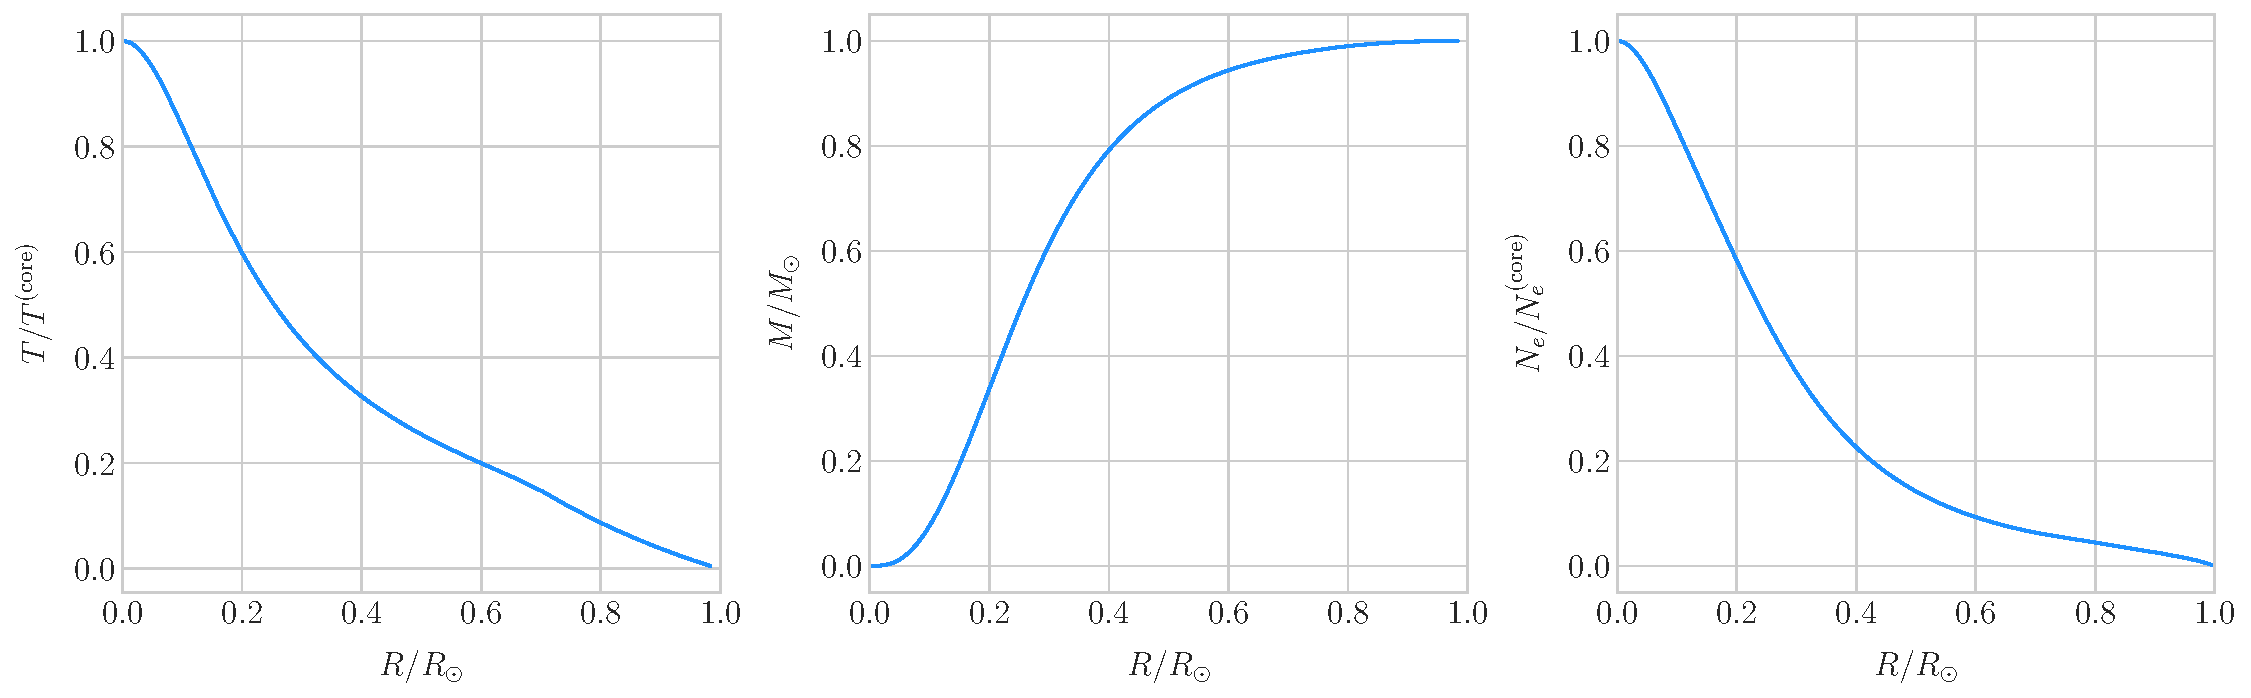
\includegraphics[width=1\linewidth]{Images/DM_Analysis/ssm_params.pdf}
	\caption[Input solar parameters used in the capture rate computation as a function of the solar radius.]{Input solar parameters used in the capture rate computation as a function of the solar radius, from left to right: temperature (with respect to the temperature at the core), mass (in solar masses) and electron number density (with respect to the electron density at the core). All quantities shown correspond to the standard solar model BS2005-OP \cite{Bahcall2004}.}
	\label{fig:ssm_params}
\end{figure}

Finally, if one assumes the DM halo velocity distribution in the galactic rest frame to be a Maxwell-Boltzmann distribution, one can write the halo velocity distribution for an observer moving at the speed of the Sun with respect to the DM rest frame as:
\begin{equation}\label{2.12}
	f_{v_{\odot}}(u_{\chi}) = \sqrt{\frac{3}{2\pi}} \frac{u_{\chi}}{v_{\odot} v_{d}} \left(\mathrm{e}^{-\frac{3(u_{\chi}-v_{\odot})^{2}}{2v_{d}^{2}}}-\mathrm{e}^{-\frac{3(u_{\chi}+v_{\odot})^{2}}{2v_{d}^{2}}}\right),
\end{equation}
where:
\begin{equation}\label{2.13}
	\omega^{2}(r) = u_{\chi}^{2} + v_{e}^{2}(r),
\end{equation}
is the DM velocity squared, $v_{\odot}$ the relative velocity of the Sun from the DM rest frame and $v_{d} \simeq \sqrt{3/2} v_{\odot}$ the velocity dispersion.

For the case of strong scattering cross sections, Eq. (\ref{2.5}) ceases to be valid, as it escalates indefinitely with the cross section. In that limit, the capture rate saturates to the case where the probability of interaction is equal to one, which can be written as \cite{Gould1987a}:
\begin{equation}\label{2.14}
	C_{\odot}^{\mathrm{geom}} = \pi R_{\odot}^{2} \left(\frac{\rho_{\chi}}{m_{\chi}}\right) \expval{v} \left(1+\frac{3}{2}\frac{v_{e}^{2}(R_{\odot})}{v_{d}^{2}}\right) \xi(v_{\odot}, v_{d}),
\end{equation}
where $\expval{v} = \sqrt{8/3\pi} v_{d}$ is the mean velocity in the DM rest frame and the factor $\xi(v_{\odot}, v_{d})$ accounts for the suppression due to the motion of the Sun:
\begin{equation}\label{2.15}
	\xi(v_{\odot}, v_{d}) = \frac{v_{d}^{2}\mathrm{e}^{-\frac{3v_{\odot}^{2}}{2v_{d}^{2}}}+\sqrt{\frac{\pi}{6}}\frac{v_{d}}{v_{\odot}}\left(v_{d}^{2}+3v_{e}^{2}(R_{\odot})+3v_{\odot}^{2}\right)\mathrm{Erf}\left(\sqrt{\frac{3}{2}}\frac{v_{\odot}}{v_{d}}\right)}{2v_{d}^{2}+3v_{e}^{2}(R_{\odot})}.
\end{equation}

Having these into account, one can write the total capture rate as a combination of both contributions, allowing a smooth transition between the two, as \cite{Bernal2012}:
\begin{equation}\label{2.16}
	C_{\odot} = C_{\odot}^{\mathrm{weak}} \left(1-\mathrm{e}^{C_{\odot}^{\mathrm{geom}}/C_{\odot}^{\mathrm{weak}}}\right).
\end{equation}

\begin{figure}[t]
	\centering
	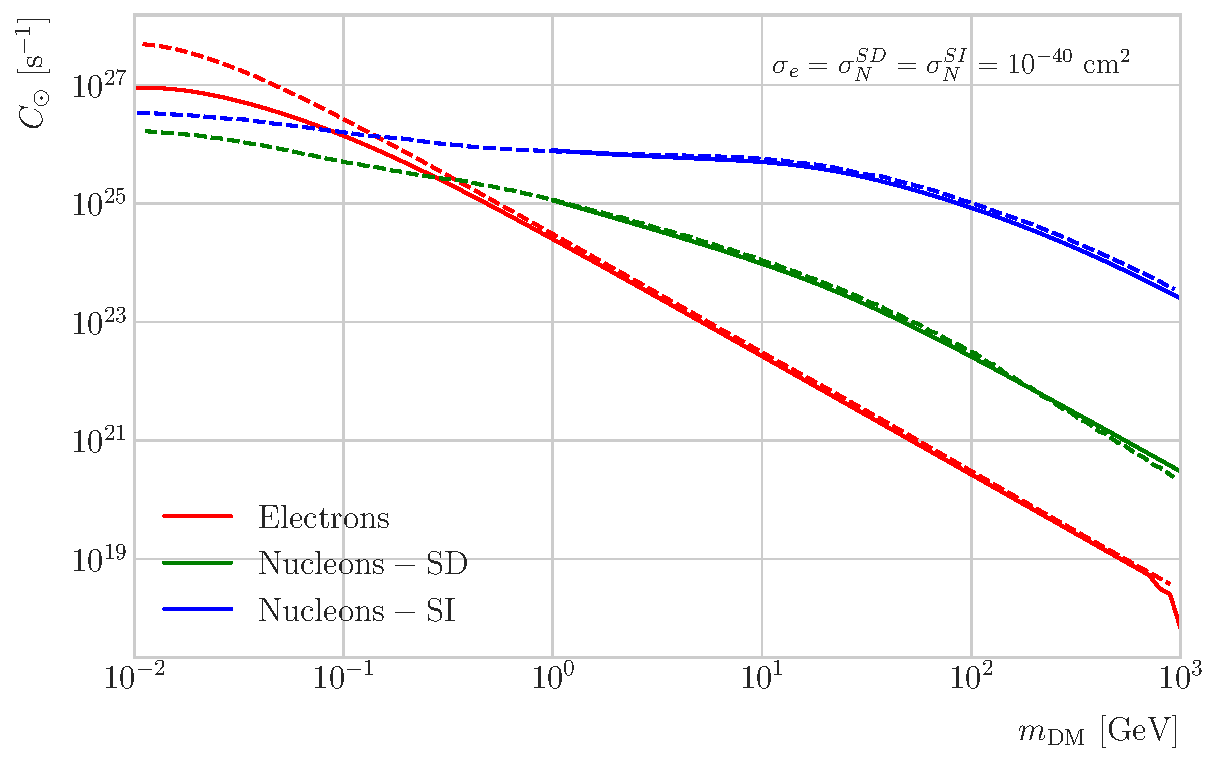
\includegraphics[width=0.9\linewidth]{Images/DM_Analysis/capture_rates.pdf}
	\caption[Capture rates as a function of the DM mass for the DM-electron interactions, SD DM-nucleons interactions, and SI DM-nucleons interactions.]{Capture rates as a function of the DM mass for the DM-electron interactions (red lines), SD DM-nucleons interactions (green lines), and SI DM-nucleons interactions (blue lines). Solid lines represent the values computed in this work while the dashed lines are the one given in Ref. \cite{Palomares2017}. All the rates are shown for a choice of scattering cross section of $\sigma_{i} = 10^{-40} \ \mathrm{cm}^{2}$.}
	\label{fig:capture_rates}
\end{figure}

I computed the capture rate from Eq. (\ref{2.16}) in the case of interactions with electrons. To do so, I used the standard solar model BS2005-OP \cite{Bahcall2004}. Fig. \ref{fig:ssm_params} shows the three parameters from the solar model that are needed for the computation, the solar temperature (left panel), mass (central panel) and electron density (right panel) profiles.

For the case of the interactions off nuclei, the computations are more convoluted as one needs to add up the contributions of the different most abundant nuclei in the Sun. Also, in contrast to the electron scenario where the form factor is trivially $|F_{e}(q)|^{2} = 1$, for any nucleus $i$ one would need to consider some appropriate nuclear density distribution (either a Gaussian approximation, a Woods-Saxon distribution, etc) which would complicate the calculations even further.

That is the reason why, at this stage of the study, I decided to take an alternative approach to the computation of the DM-nucleus capture rates. I used the \texttt{DarkSUSY} software, that allows us to compute these quantities performing a full numerical integration over the momentum transfer of the form factors \cite{Bringmann2018}. The default standard solar model used by \texttt{DarkSUSY} is BP2000\footnote{This is what they say in their manual, but I fear it is somewhat outdated. It appears to me this model is relatively old and do not see why they are not using others like \cite{Bahcall2004}. Maybe one can double-check in the code to make sure.} \cite{Bahcall2000}.

In Fig. \ref{fig:capture_rates} I show the results I obtain for the capture rates, for the case of interactions off electrons (red solid line), SD (green solid line) and SI (blue solid line) interactions of nucleons. In all cases I use a value of the scattering cross sections of $\sigma_{i} = 10^{-40} \ \mathrm{cm}^{2}$. Note here one of the limitations of the \texttt{DarkSUSY} approach, one can not extend the computation below $m_{\mathrm{DM}} = 1 \ \mathrm{GeV}$. Nevertheless, this is not something to worry about in this case, as I will discuss next. As a comparison, I added also the values computed in Ref. \cite{Palomares2017} (same color scheme, dashed lines). One can see there is good agreement between these and the \texttt{DarkSUSY} computation of the SD and SI interactions for $m_{\mathrm{DM}} \geq 1 \ \mathrm{GeV}$. In this regime their computations also matches quite well the results for the electron capture rate. However, these start to differ significantly below $m_{\mathrm{DM}} = 1 \ \mathrm{GeV}$, being their estimate up to a factor of $5$ bigger than ours for low masses. This could be due to the use of a different solar model in the calculation.

Let me comment briefly about the assumption I made before about not including an evaporation term in the Boltzmann equation. If I include this term in the equation, which is proportional to the number of DM particles, the equilibrium solution takes the form:
\begin{equation}\label{2.17}
	N_{DM}^{eq} = \sqrt{\frac{C_{\odot}}{A_{\odot}}} \frac{1}{\kappa + \frac{1}{2} E_{\odot} \tau_{eq}},
\end{equation}
where $E_{\odot}$ is the total evaporation rate, $\tau_{eq}$ is the equilibrium time in the absence of evaporation:
\begin{equation}\label{2.18}
	\tau_{eq} = \frac{1}{\sqrt{C_{\odot} A_{\odot}}},
\end{equation}
and $\kappa$ is defined as:
\begin{equation}\label{2.19}
	\kappa \equiv \sqrt{1+\left(\frac{E_{\odot}\tau_{eq}}{2}\right)^{2}}.
\end{equation}

Now, it is easy to proof that in the case evaporation dominates $\kappa \gg 1$ and therefore:
\begin{equation}\label{2.20}
	N_{DM}^{eq} \simeq \frac{C_{\odot}}{E_{\odot}}.
\end{equation}
In contrast, if evaporation is irrelevant $\kappa \simeq 1$ and one recovers Eq. (\ref{2.2}).

In this way, one can define the evaporation mass as the mass for which the number of DM particles in equilibrium approaches Eq. (\ref{2.20}) at $10 \%$ level:
\begin{equation}\label{2.21}
	\left| N_{DM}^{eq}(m_{\mathrm{evap}}) - \frac{C_{\odot}(m_{\mathrm{evap}})}{E_{\odot}(m_{\mathrm{evap}})} \right| = 0.1 N_{DM}^{eq}(m_{\mathrm{evap}}).
\end{equation}
This can be regarded as the minimum testable mass one can reach using the annihilation products of the DM in the Sun.

It was reported in Ref. \cite{Palomares2017} that, in the case of both SD and SI DM interactions off nuclei, this value ranges from $2$ to $4 \ \mathrm{GeV}$ depending on the specific scattering cross section value, compatible with the usual assumptions in the literature. What is interesting is the case of the electron capture. It was found that, when one applies a cutoff in the velocity distribution of the DM trapped in the Sun slightly below the escape velocity, the evaporation mass for the DM-electron interaction decreases remarkably. For a moderate choice of $v_{c}(r) = 0.9 v_{e}(r)$ one gets an evaporation mass of around $200$ to $600 \ \mathrm{MeV}$. This possibility opens a region of the parameter space that could be tested with the next generation of neutrino detectors.

\section{Neutrino flux from DM annihilations}
\label{sec:dm_analysis_flux}

When WIMPs annihilate inside the Sun a flux of high-energy neutrinos is expected from heavy quarks, gauge bosons and $\tau^{+}\tau^{-}$ final states, which decay before losing energy in the dense solar medium \cite{Rott2012}. These produce a continuous neutrino spectra up to $E_{\nu} \sim m_{\chi}$. In the case of direct annihilation into neutrinos, one would have a monochromatic flux with $E_{\nu} = m_{\chi}$. This kind of signal has been extensively studied  in the literature, allowing to put strong limits on the SD WIMP-proton cross section for large $m_{\chi}$. However, the number of high-energy neutrinos per WIMP annihilation is small and the spectrum depends on the unknown final state. Moreover, although background rejection is easier for large $m_{\chi}$, neutrinos with $E_{\nu} \gtrsim 100 ~ \mathrm{GeV}$ are significantly attenuated by interactions in the Sun.

Nevertheless, most WIMP annihilation final states eventually produce a low-energy neutrino spectrum.  In this case one does not just consider the more massive final states but also annihilations into $e^{+}e^{-}$, $\mu^{+}\mu^{-}$ and light quarks \cite{Bernal2012}. In particular, light mesons would be produced and stopped in the dense medium, thus decaying at rest and producing a monoenergetic neutrino signal. The decay-at-rest of kaons will produce a $\nu_{\mu}$ flux with $E_{\nu} = 236 ~ \mathrm{MeV}$, while in the case of pions one would have $E_{\nu}  = 29.8 ~ \mathrm{MeV}$. In practice, only the $K^{+}$ and $\pi^{+}$ contribute to these signals, as the $K^{-}$ and $\pi^{-}$ are usually Coulomb-captured in an atomic orbit and get absorbed by the nucleus. There is also a low-energy neutrino signal coming from muon decays, which are produced in kaon or pion decays, leptonic decays of other hadrons and heavy leptons or even directly from WIMP annihilations. These can decay at rest and contribute to the previous low-energy neutrino flux with a well known spectrum below $52.8 ~ \mathrm{MeV}$.

These monoenergetic $\mathrm{MeV}$ neutrinos were previously considered undetectable but, due to the large yield, the known spectra and the modern advances in the detector technology, these low-energy neutrino flux can be a good probe of the SD WIMP-proton cross section in standard solar WIMP capture scenario, as it is sensitive to low WIMP masses and insensitive to the particular final state. A good place to look for these signals are next-generation neutrino experiments such as DUNE.

\section{Computing limits from solar neutrino fluxes}
\label{sec:dm_analysis_limits}

\begin{figure}[t]
	\centering
	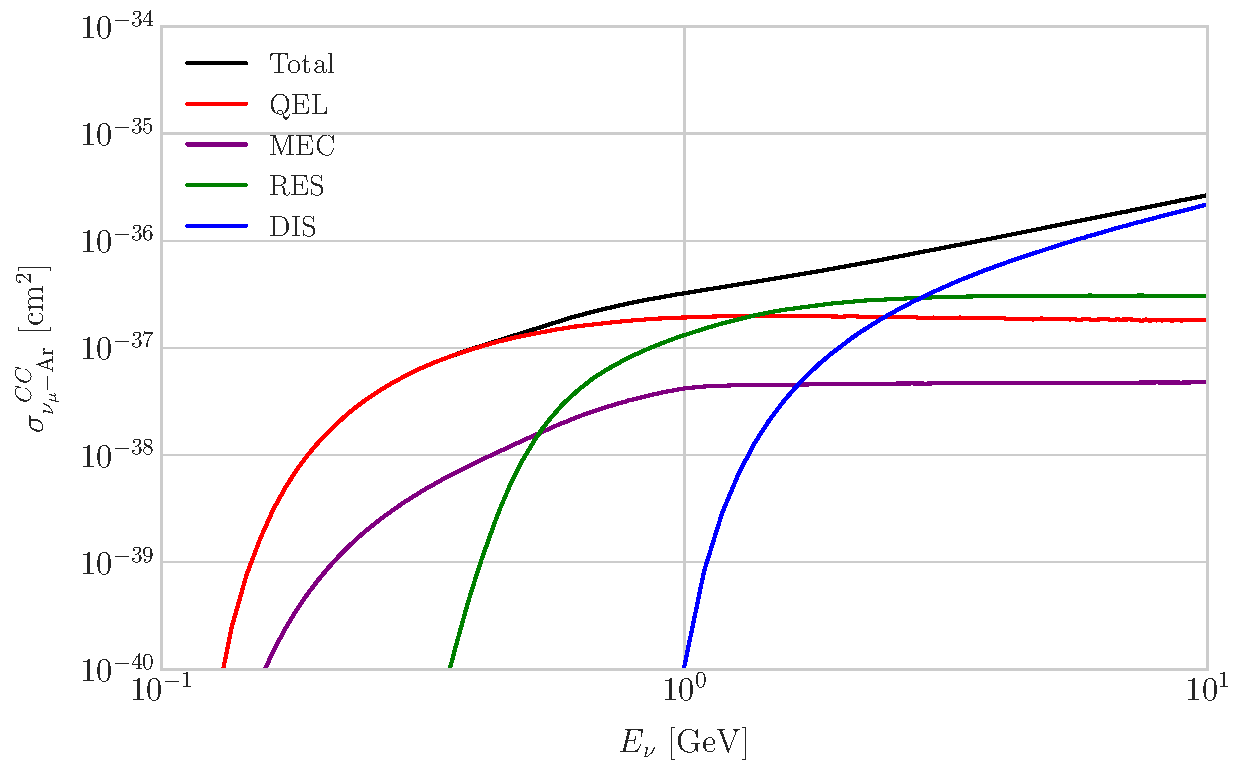
\includegraphics[width=0.9\linewidth]{Images/DM_Analysis/nu_Ar_xsection}
	\caption[\texttt{NuWro} computed $\nu_{\mu}-\ce{^{40}Ar}$ charged-current scattering cross section as a function of the neutrino energy.]{\texttt{NuWro} computed $\nu_{\mu}-\ce{^{40}Ar}$ charged-current scattering cross section as a function of the neutrino energy. The black line shows to the total cross section, whereas the others correspond to the different contributions (in red quasi-elastic scattering, in green resonant pion exchange, in blue deep inelastic scattering and in purple meson exchange current).}
	\label{fig:nu_Ar_xsection}
\end{figure}

The first step to use these fluxes to search for DM in the Sun is to determine the expected number of atmospheric background events. For a given exposure, after directionality selection has been applied, this can be written as:
\begin{equation}\label{4.1}
	N_{B} = \eta_{B} \int \mathrm{d}\Omega \int_{E_{min}}^{E_{max}} \mathrm{d}E_{\nu} \ \frac{\mathrm{d}^{2}\Phi_{atm}^{\mu}}{\mathrm{d}E_{\nu} \mathrm{d}\Omega} \times \left(A_{eff}^{(\mu)}(E_{\nu}) T\right),
\end{equation}
where $\eta_{B}$ is the background efficiency, $E_{min}$ and $E_{max}$ the minimum and maximum energies to integrate over, $\mathrm{d}^{2}\Phi_{atm}^{\mu} / \mathrm{d}E_{\nu} \mathrm{d}\Omega$ the differential flux of atmospheric muon neutrinos, $A_{eff}^{(\mu)}$ is the effective area of DUNE to muon neutrinos, and $T$ is the exposure time. The effective area can be expressed as the product of the neutrino-nucleus scattering cross section and the number of nuclei in the fiducial volume of the detector. This way, for DUNE we have:
\begin{equation}\label{4.2}
	A_{eff}^{(\mu)}(E_{\nu}) = (6.0 \times 10^{-10} \ \mathrm{m}^{2}) \left(\frac{\sigma_{\nu - \mathrm{Ar}}^{(\mu)}(E_{\nu})}{10^{-38} \ \mathrm{cm}^{2}}\right) \left(\frac{M_{target}}{40 \ \mathrm{kT}}\right),
\end{equation}
where $\sigma_{\nu - \mathrm{Ar}}^{(\mu)}$ is the $\nu_{\mu}-\ce{^{40}Ar}$ charged-current scattering cross section. In Fig. \ref{fig:nu_Ar_xsection} I show the computed value of the cross section as a function of the neutrino energy $E_{\nu}$, in the range of interest both for the atmospheric background and signal events. It was computed using the \texttt{NuWro} Monte Carlo neutrino event generator \cite{Golan2012}, including the CC contributions of the quasi-elastic scattering (red line), resonant pion exchange (green line), deep inelastic scattering (blue line) and meson exchange current (purple line).

The background rejection will depend on the resolution of the detector and the selection one applies on the events. A geometry argument can be used to estimate the maximum background rejection one can achieve in this case, considering one can efficiently discriminate all events coming from a direction different from that of the Sun. In that case, the optimal background efficiency will simply be the relative angular coverage of the Sun. Taking the angular diameter of the Sun as seen from the Earth to be $0.5^{\circ}$, I have:
\begin{equation}\label{4.3}
	\eta_{B}^{(opt)} \approx \frac{\pi \left(\frac{0.5}{2}\right)^{2}}{360 \times 180} \simeq 3.03 \times 10^{-6}.
\end{equation}
This value gives an optimistic estimate of the number of background events. However, it can be regarded as an upper limit, as it represents the best case scenario.

In Fig. \ref{fig:homestake_fluxes} I show the fluxes of atmospheric neutrinos at the Homestake mine during solar minimum, taken from Ref. \cite{Honda2015}. The values are averaged over the two angular directions. In blue I have the flux of muon neutrinos while in red I indicate the flux of electron neutrinos. Additionally, the dashed lines correspond to both antineutrino species.

Using these values for the muon neutrino and the corresponding total CC cross section, one can compute the total number of expected background events by integrating over the given energy range. For this I choose the range for DUNE specified in \cite{DUNE2020TDR2}, $E_{min} = 10^{-1} \ \mathrm{GeV}$ and $E_{max} = 10 \ \mathrm{GeV}$. Taking all these into account, I find the total number of background events to be:
\begin{equation}\label{4.4}
	N_{B} \simeq  \eta_{B} \times \left(3.827 \times 10^{4}\right) \times \left(\frac{\mathrm{exposure}}{400 \ \mathrm{kT \ yr}}\right).
\end{equation}

\begin{figure}[t]
	\centering
	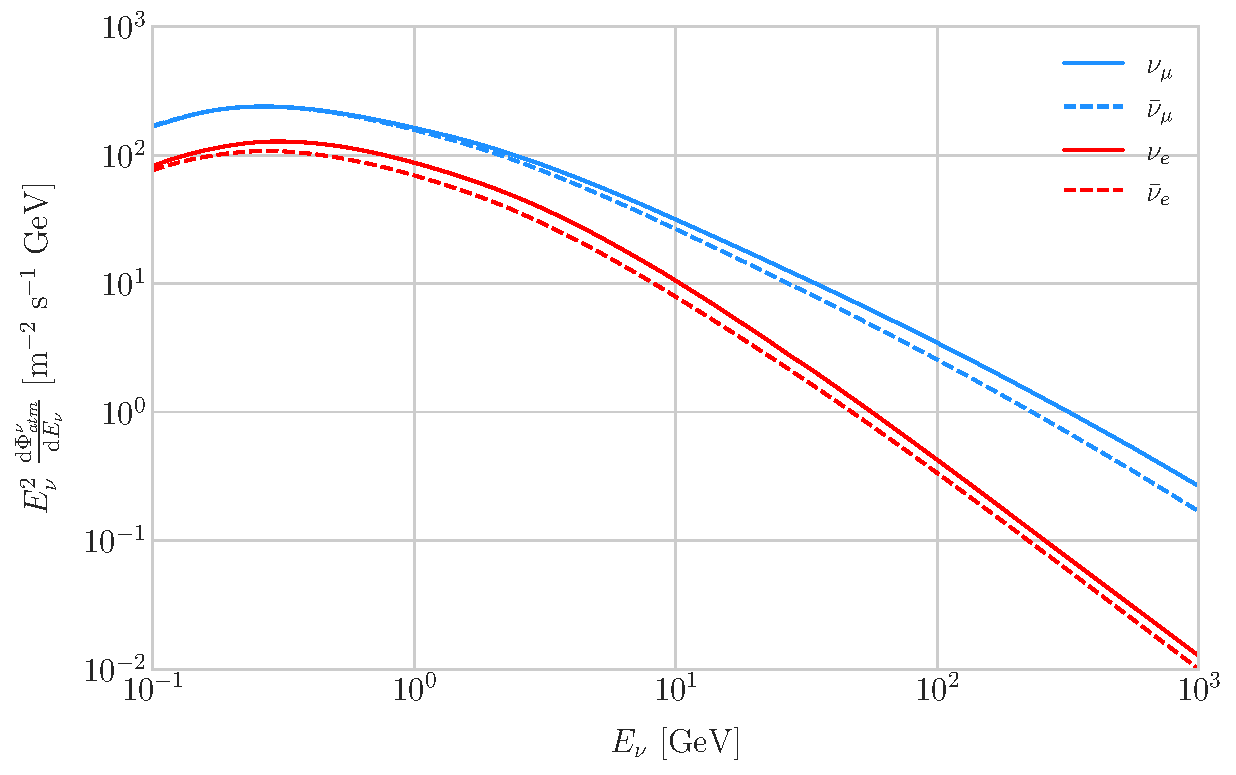
\includegraphics[width=0.9\linewidth]{Images/DM_Analysis/homestake_fluxes}
	\caption[Expected atmospheric neutrino flux as a function of the neutrino energy $E_{\nu}$ at Homestake at solar minimum.]{Expected atmospheric neutrino flux as a function of the neutrino energy $E_{\nu}$ at Homestake at solar minimum, taken from Ref. \cite{Honda2015}. The blue solid (dashed) line correspond to muon neutrinos (antineutrinos) and the red solid (dashed) line correspond to electron neutrinos (antineutrinos).}
	\label{fig:homestake_fluxes}
\end{figure}

To estimate the sensitivity of DUNE to this kind of signals, one can consider a hypothetical data set where the number of observed neutrinos is taken to be the expected number of background events rounded to the nearest integer, $N_{obs} = \mathrm{round}(N_{B})$ \cite{Cowan2010}. Now, if I assume that the number of signal and background events seen by DUNE are given by Poisson distributions with means equal to the expected number of signal and background events, $N_{S}$ and $N_{B}$, one can denote by $N_{S}^{90}$ to the number of expected signal events such that the probability of having an experimental run with a number of events greater than $N_{obs}$ is $90\%$. This number can be obtained as the numerical solution to the equation:
\begin{equation}\label{4.5}
	1 - \frac{\Gamma\left(N_{obs}+1, N_{S}^{90}+N_{B}\right)}{N_{obs}!} = 0.9,
\end{equation}
where $\Gamma(x,y)$ is the upper incomplete gamma function.

The number of signal events is related to the neutrino flux from DM annihilations in a similar way as the background events to the atmospheric neutrino flux. In this case I have:
\begin{equation}\label{4.6}
	N_{S} = \eta_{S} \ \Gamma_{A}^{eq} \int_{z_{min}}^{z_{max}} \mathrm{d}z \ \frac{\mathrm{d}N_{\nu}}{\mathrm{d}A \mathrm{d}N_{A} \mathrm{d}z}  \times \left(A_{eff}^{\mu}(z) T\right),
\end{equation}
where $\eta_{S}$ is the signal efficiency, $\Gamma_{A}^{eq}$ is the total annihilation rate of DM particles at equilibrium, $\Gamma_{A}^{eq} = A_{\odot} \left(N_{DM}^{eq}\right)^{2}$, $z_{min}$ and $z_{max}$ the minimum and maximum relative energies to integrate over (given by $z_{min, max} = E_{min, max}/m_{\mathrm{DM}}$ for each $m_{\mathrm{DM}}$) and $\mathrm{d}N_{\nu}/\mathrm{d}A \mathrm{d}N_{A} \mathrm{d}z$ the muon neutrino flux per DM annihilation in the Sun.

Having obtained $N_{S}^{90}$ one can use the relation in Eq. (\ref{4.6}) to compute $\Gamma_{A}^{eq,90}$ for different values of the DM mass. Then, I can directly translate those values into the projected sensitivities for DUNE to the DM scattering cross sections, for a given exposure. The relation between the annihilation rate and the DM-nucleon cross section comes from the equilibrium condition through the solar DM capture rate, discussed above.

\section{Example: Kaluza-Klein Dark Matter}
\label{sec:dm_analysis_kk_dm}

Even though there are plenty of BSM theories which provide viable dark matter candidates, Kaluza-Klein type of models \cite{Kaluza1921, Klein1926} within the universal extra dimensions (UED) paradigm naturally predict the existence of a massive, stable particle that can play the role of the dark matter. In the UED scenario all the SM fields can propagate in one or more compact extra dimensions \cite{Appelquist2000}, as opposed to the idea of brane worlds \cite{Arkani-Hamed1998, Randall1999}, where just gravity can propagate in the bulk while SM particles live at fixed points.

Furthermore, in UED there is no violation of the translational invariance along the extra dimensions, thus leading to degenerate KK modes masses  and also the conservation of the KK number in the effective four dimensional theory. At loop level, radiative corrections and boundary terms shift the masses of the KK modes and break KK number conservation into a KK parity. As a result, this theory only contains interactions between an even number of odd KK modes and therefore the lightest among the first KK excitations will be stable. This particle is usually denoted as the lightest Kaluza-Klein particle (LKP) and its mass is proportional to $1/R$, being $R$ the size of the extra dimension.

\begin{figure}
	\centering
	\begin{subfigure}{0.4\textwidth}
		\centering
		\tikz{
			\begin{feynman}
				% left side: for i1 -- a -- b -- f1
				\vertex                         (i1) {\(B^{1}\)};
				\vertex [below right=2cm of i1] (a);
				\vertex [below=1.5cm of a]      (b);
				\vertex [below left=1.5cm of b] (i2){\(B^{1}\)};

				% right side: i2(e+) and f2(e-)
				\vertex [right=3cm of i1]       (f1) {\(f\)};
				\vertex [right=3cm of i2]       (f2) {\(\bar{f}\)};


				\diagram* {
					% left side
					(i1) -- [boson] (a),% e-
					(a) -- [anti fermion, edge label'=\(f^{1}\)](b),
					(b) -- [anti fermion](f2),% e+
					
					% cross-overs at the right side
					(i2) -- [boson] (b),
					(a) -- [fermion] (f1)
				};

			\end{feynman}
		}
	\end{subfigure}
	\begin{subfigure}{0.4\textwidth}
		\centering
		\tikz{
			\begin{feynman}
				% left side: for i1 -- a -- b -- f1
				\vertex                         (i1) {\(B^{1}\)};
				\vertex [below right=2cm of i1] (a);
				\vertex [below=1.5cm of a]      (b);
				\vertex [below left=1.5cm of b] (i2){\(B^{1}\)};

				% right side: i2(e+) and f2(e-)
				\vertex [right=3cm of i1]       (f1) {\(f\)};
				\vertex [right=3cm of i2]       (f2) {\(\bar{f}\)};


				\diagram* {
					% left side
					(i1) -- [boson] (b),% e-
					(a) -- [anti fermion, edge label=\(f^{1}\)](b),
					(b) -- [anti fermion](f2),% e+
					
					% cross-overs at the right side
					(i2) -- [boson] (a),
					(a) -- [fermion] (f1)
				};

			\end{feynman}
		}
	\end{subfigure}
	\caption{Feynman diagrams for $B^{1}$$B^{1}$ annihilation into SM fermions.}
\end{figure}

\begin{figure}
	\centering
	\begin{subfigure}{0.25\textwidth}
		\centering
		\tikz{
			\begin{feynman}
				% left side: for i1 -- a -- b -- f1
				\vertex                         (i1) {\(B^{1}\)};
				\vertex [below right=2cm of i1] (a);
				\vertex [below=1.5cm of a]      (b);
				\vertex [below left=1.5cm of b] (i2){\(B^{1}\)};

				% right side: i2(e+) and f2(e-)
				\vertex [right=3cm of i1]       (f1) {\(\phi\)};
				\vertex [right=3cm of i2]       (f2) {\(\phi\)};


				\diagram* {
					% left side
					(i1) -- [boson] (a),% e-
					(a) -- [scalar, edge label'=\(\phi^{1}\)](b),
					(b) -- [scalar](f2),% e+
					
					% cross-overs at the right side
					(i2) -- [boson] (b),
					(a) -- [scalar] (f1)
				};

			\end{feynman}
		}
	\end{subfigure}
	\begin{subfigure}{0.25\textwidth}
		\centering
		\tikz{
			\begin{feynman}
				% left side: for i1 -- a -- b -- f1
				\vertex                         (i1) {\(B^{1}\)};
				\vertex [below right=2cm of i1] (a);
				\vertex [below=1.5cm of a]      (b);
				\vertex [below left=1.5cm of b] (i2){\(B^{1}\)};

				% right side: i2(e+) and f2(e-)
				\vertex [right=3cm of i1]       (f1) {\(\phi\)};
				\vertex [right=3cm of i2]       (f2) {\(\phi\)};


				\diagram* {
					% left side
					(i1) -- [boson] (b),% e-
					(a) -- [scalar, edge label=\(\phi^{1}\)](b),
					(b) -- [scalar](f2),% e+
					
					% cross-overs at the right side
					(i2) -- [boson] (a),
					(a) -- [scalar] (f1)
				};

			\end{feynman}
		}
	\end{subfigure}
	\begin{subfigure}{0.25\textwidth}
		\centering
		\tikz{
			\begin{feynman}
				% left side: for i1 -- a -- b -- f1
				\vertex                         (i1) {\(B^{1}\)};
				\vertex [below right=2cm of i1] (a);
				\vertex [below left=1.5cm of a] (i2){\(B^{1}\)};

				% right side: i2(e+) and f2(e-)
				\vertex [right=3cm of i1]       (f1) {\(\phi\)};
				\vertex [right=3cm of i2]       (f2) {\(\phi\)};


				\diagram* {
					% left side
					(i1) -- [boson] (a),% e-
					(a) -- [scalar](f2),% e+
					
					% cross-overs at the right side
					(i2) -- [boson] (a),
					(a) -- [scalar] (f1)
				};

			\end{feynman}
		}
	\end{subfigure}
	\caption{Feynman diagrams for $B^{1}$$B^{1}$ annihilation into a Higgs boson pair.}
\end{figure}

A viable DM candidate needs to be electrically neutral and non-baryonic, therefore good candidates among the first Kaluza-Klein excitations would be the KK neutral gauge bosons and the KK neutrinos \cite{Servant2002}. Another possible candidate is the first KK excitation of the graviton, which receives negligible radiate contributions and therefore has a mass almost equal to $1/R$, but it has been shown that the lightest eigenstate from the mixing of the gauge mass states $\left(B^{1}, W_{3}^{1}\right)$ would be lighter, as $B^{1}$ and $W_{3}^{1}$ receive negative radiate corrections \cite{Cheng2002}. It is also understood that, when these corrections become sizeable, the eigenstates become approximately pure $B^{1}$ and $W_{3}^{1}$ states as the Weinberg mixing angle grows small with the KK number \cite{Cheng2002}. In that case, the LKP can be well-approximated as being entirely $B^{1}$.

\begin{figure}[t]
	\centering
	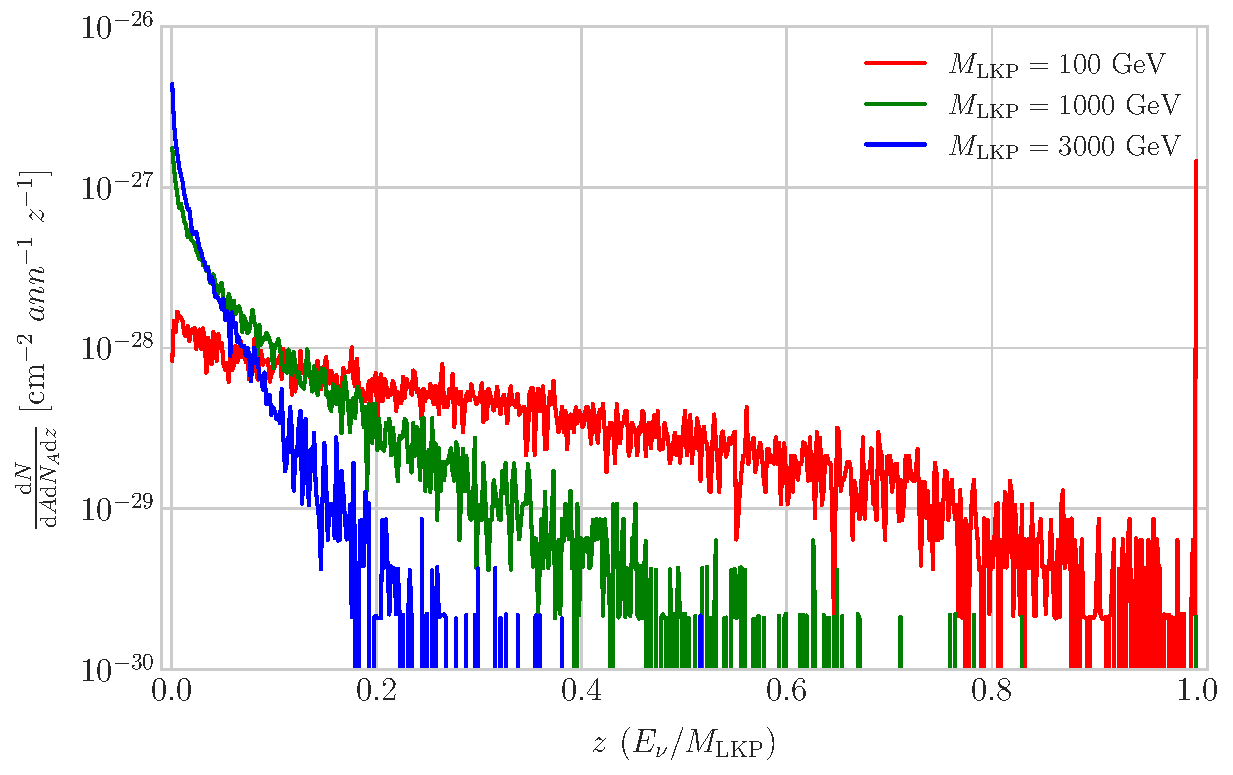
\includegraphics[width=0.9\linewidth]{Images/DM_Analysis/KK_nu_flux}
	\caption[Computed spectra of muon neutrinos at the DUNE FD site from $B^{1}$ annihilations in the Sun for various values of $M_{\mathrm{LKP}}$.]{Computed spectra of muon neutrinos at the DUNE FD site from $B^{1}$ annihilations in the Sun for three different values of $M_{\mathrm{LKP}}$, plotted in relative energy units for legibility.}
	\label{fig:KK_nu_flux}
\end{figure}

I need to compute the neutrino flux produced by the annihilations of the LKP in the core of the Sun, taking into account their propagation in the solar medium, as well as neutrino oscillations.  To this end I used \texttt{WimpSim} \cite{Blennow2007, WimpSim} to generate one million annihilation events in the Sun over a time span of four years and propagate them to the DUNE FD location (44$^{\circ} $ 20' N, 103$^{\circ} $ 45' W), for different values of $M_{\mathrm{LKP}}$. In Fig. \ref{fig:KK_nu_flux} I show the obtained muon neutrino spectra arriving to the detector from LKP annihilations in the Sun, per unit area and per annihilation, plotted in relative energy units for different values of the mass. As one could expect the spectra get steeper the higher is the mass, due to the absorption of high-energy neutrinos in the solar medium. Also, one can see  the peak at $z=1$ due to the direct annihilation into neutrinos $\chi \chi \rightarrow \nu \bar{\nu}$.

Now, one can estimate the sensitivity of DUNE to this particular model by using the methods I previously discussed. To begin with, I will use the optimistic estimation of the background efficiency in Eq. (\ref{4.3}) to get an upper bound. Using it, one can directly compute the number of expected background events to be $N_{B} = 0.11$ for an exposure of $400 \ \mathrm{kT}  \ \mathrm{yr}$. Then, Eq. (\ref{4.5}) give us a value of $N_{S}^{90} = 2.20$ for the $90\%$ exclusion number of expected signal events. By using the \texttt{NuWro} generated cross sections and the computed neutrino fluxes from $B^{1}$ annihilations in the Sun I can estimate the limits on the SD and SI DM-nucleus cross section using the relation in Eq. (\ref{2.2}) and the capture rates I computed with \texttt{DarkSUSY}.

\begin{figure}[t]
	\centering
	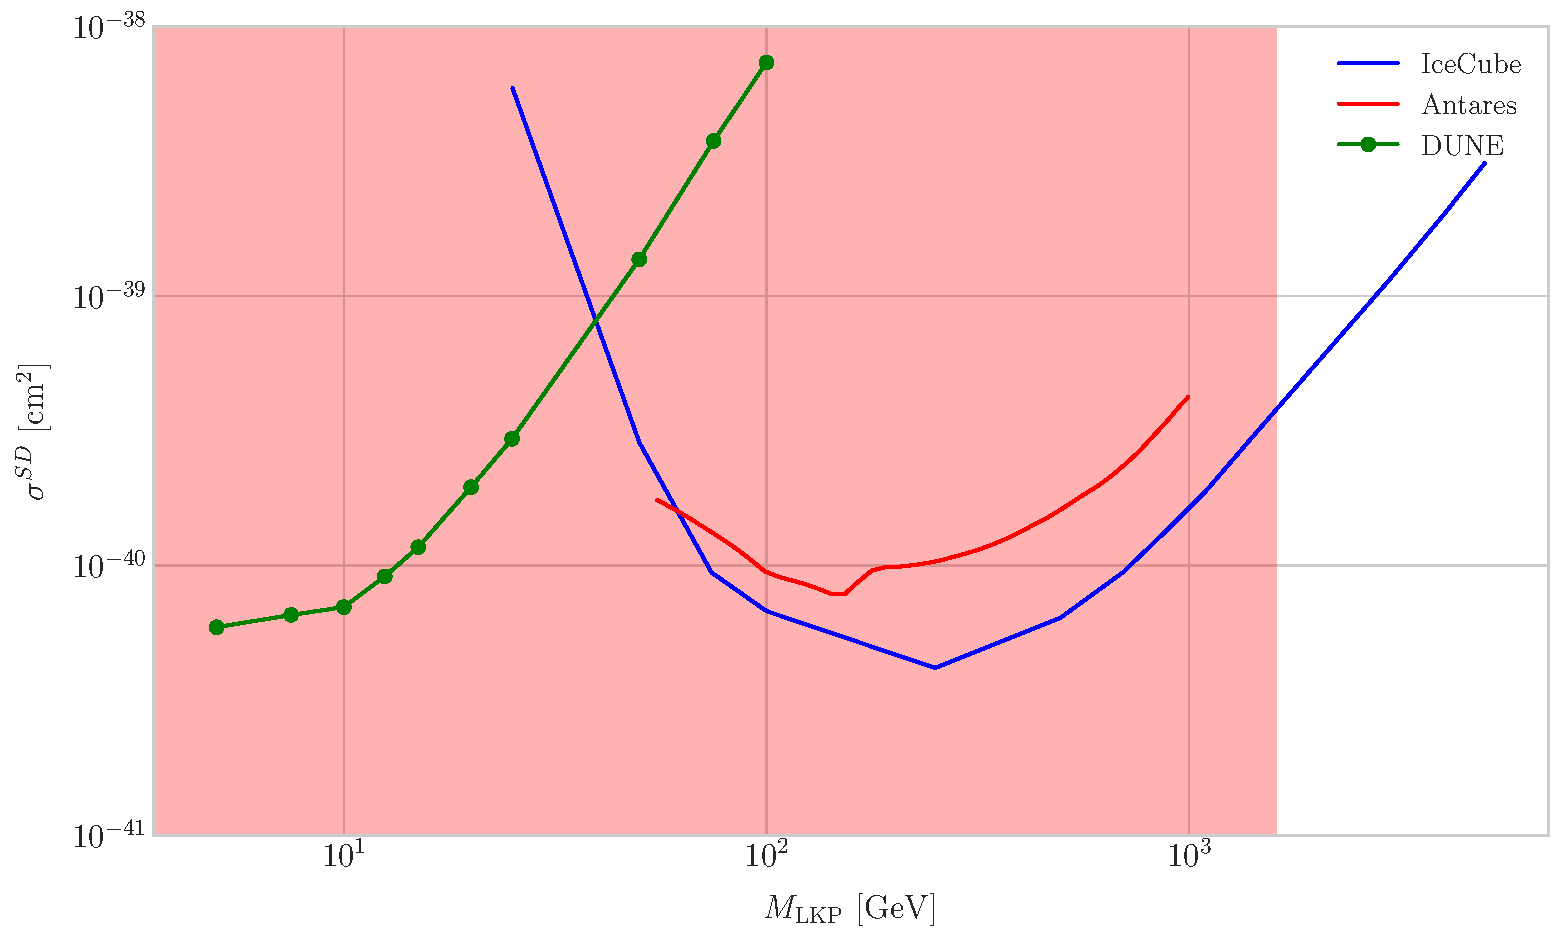
\includegraphics[width=0.9\linewidth]{Images/DM_Analysis/kk_xsection_sd_bounds}
	\caption[Projected 90\% confidence level upper limit for DUNE (400 kT yr) on the spin-dependent $B^{1}$-proton scattering cross section as a function of $M_{\mathrm{LKP}}$.]{Projected 90\% confidence level upper limit for DUNE (400 kT yr) on the spin-dependent $B^{1}$-proton scattering cross section as a function of $M_{\mathrm{LKP}}$ (green dots). I also show the previous limits from IceCube \cite{Bernadich2019} (blue line) and Antares \cite{Zornoza2012} (red line) on the LKP cross section. The shaded area represents the disfavoured region (at 95\% confidence level) on the mass of the LKP from LHC data \cite{Deutschmann2017}.}
	\label{fig:kk_xsection_sd_bounds}
\end{figure}

In Fig. \ref{fig:kk_xsection_sd_bounds} I show the projected sensitivity for DUNE on the spin-dependent $B^{1}$-proton scattering cross section versus the mass of the DM particle, for a exposure of $400 \ \mathrm{kT}  \ \mathrm{yr}$ (green dots). I also include the previous results from IceCube \cite{Bernadich2019} (blue line) and Antares \cite{Zornoza2012} (red line). The shaded area represents the disfavoured region from combined searches for UED by ATLAS and CMS \cite{Deutschmann2017}.

From the experimental point of view, this estimation lacked a detailed simulation of the detector response and thus this must be consider as a mere optimistic sensitivity computation. However, it shows the potential of DUNE to constrain this kind of exotic scenarios, showing the region where it will be in a position to compete with other neutrino telescopes. A more detailed analysis is needed if I am to make a realistic estimation. Even though the region of the parameter space where DUNE would be sensitive to this particular model is quite constrained by collider searches \cite{Deutschmann2017} and other rare decay measurements \cite{Haisch2007, Freitas2008}, it still constitutes an alternative indirect probe.

\section{High energy DM neutrino signals}
\label{sec:dm_analysis_high_e_nu}

\begin{figure}[t]
	\centering
	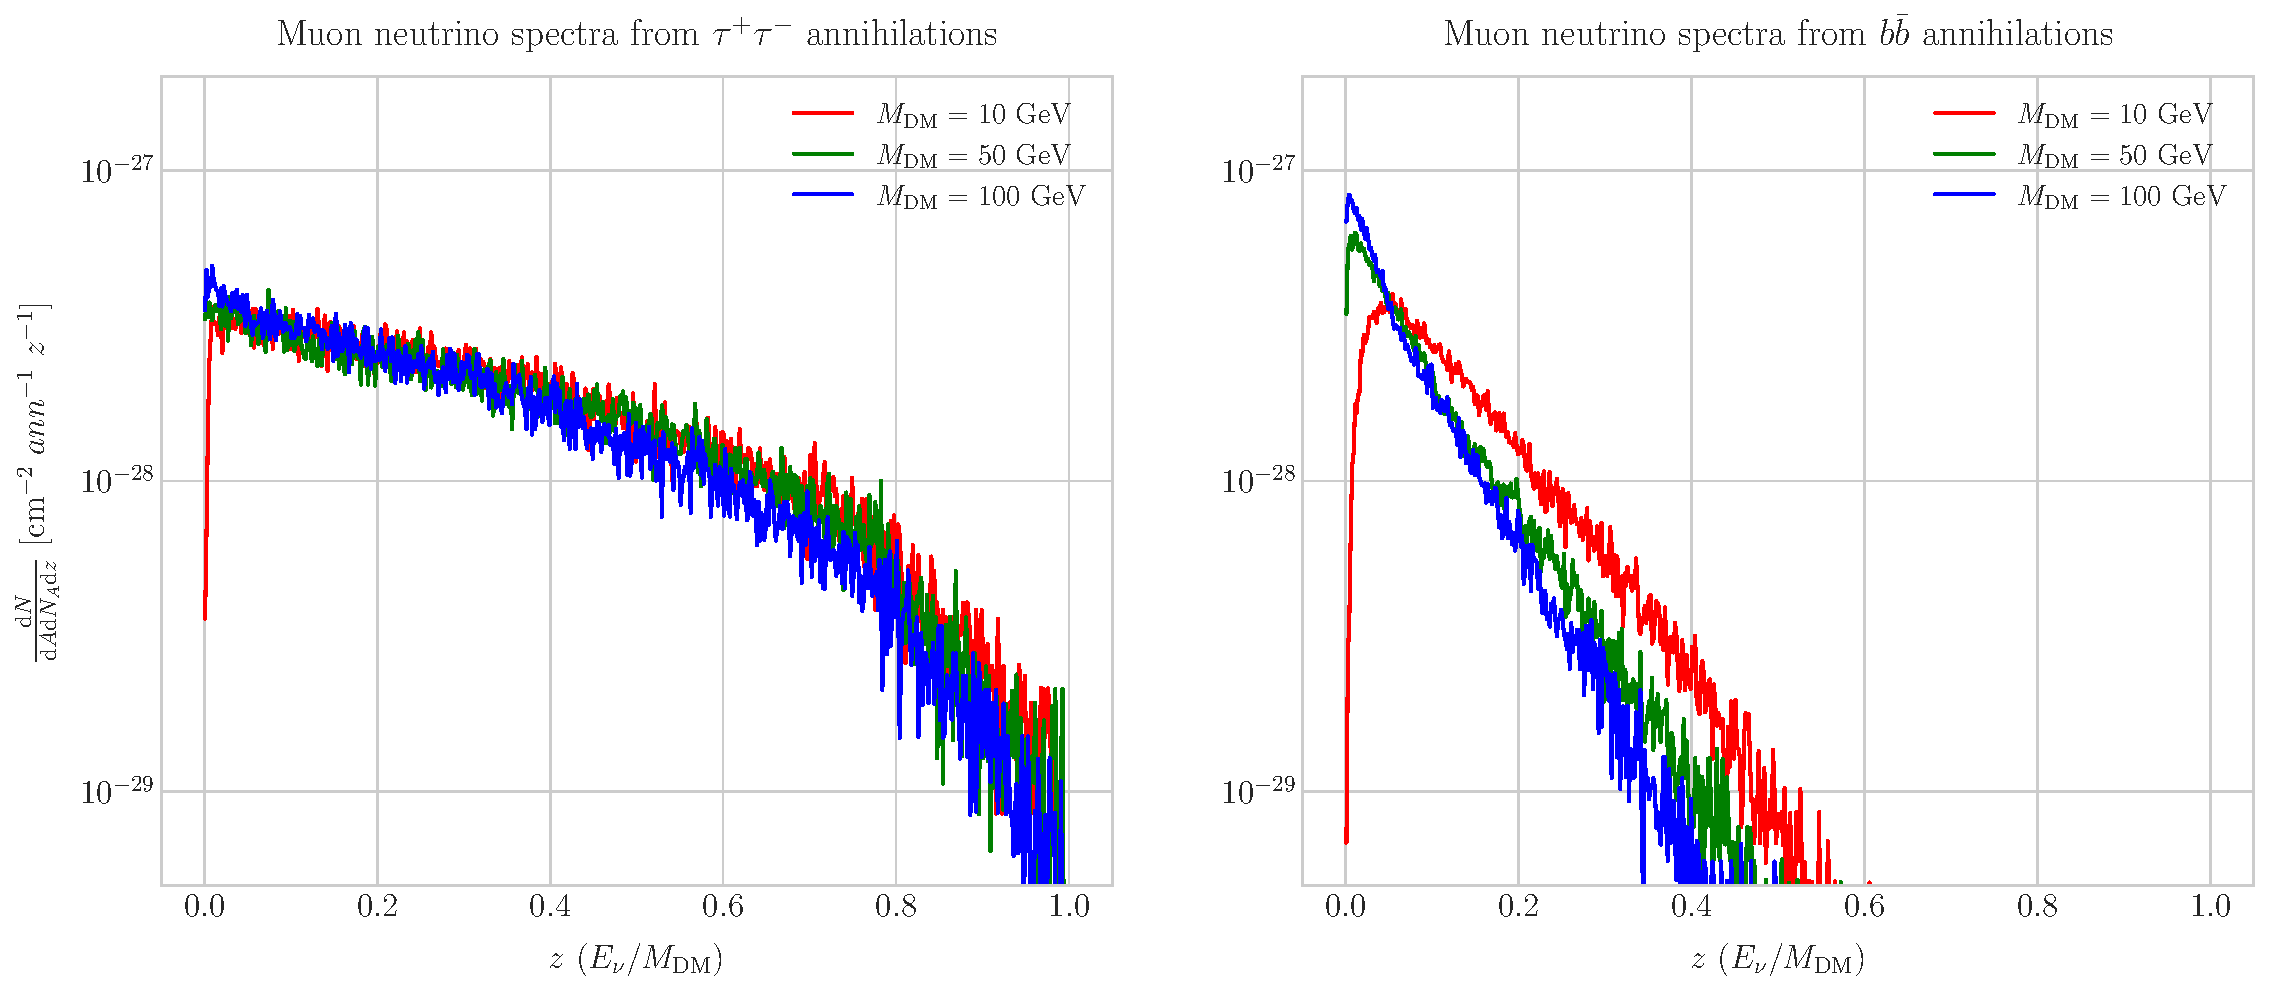
\includegraphics[width=1\linewidth]{Images/DM_Analysis/solardm_nu_mu_spectra.pdf}
	\caption[Computed spectra of muon neutrinos at the DUNE FD site from $\tau^{+} \tau^{-}$ and $b\bar{b}$ annihilations in the Sun for different DM masses.]{Computed spectra of muon neutrinos at the DUNE FD site from $\tau^{+} \tau^{-}$ (left panel) and $b\bar{b}$ (right panel) annihilations in the Sun for the DM masses $m_{\mathrm{DM}} = 10 \ \mathrm{GeV}$ (red line), $50 \ \mathrm{GeV}$ (green line) and $100 \ \mathrm{GeV}$ (blue line), plotted in relative energy units.}
	\label{fig:solardm_nu_mu_spectra}
\end{figure}

To have better estimates on the capability of the DUNE FD to constrain the parameter space of DM using solar neutrino fluxes, I need to start accounting for the detector resolution effects and the topologies of the different signatures. As a starting point, I will focus on specific annihilation channels. For the case of DUNE, the relevant ones are mainly the hard channels $\tau^{+} \tau^{-}$ and $\nu \bar{\nu}$ and the soft channel $b\bar{b}$. These are the open annihilation channels for relatively low mass WIMPs that will actually give neutrino fluxes. Other channels, like $W^{+} W^{-}$ and $ZZ$, are open for more massive WIMPs, but those will produce usually a higher energy neutrino flux that will be out of reach for DUNE (usually the maximum neutrino energy is taken to be $E_{max} = 10 \ \mathrm{GeV}$).

In Fig. \ref{fig:solardm_nu_mu_spectra} I show the \texttt{WimpSim} \cite{Blennow2007, WimpSim} generated muon neutrino spectra at the DUNE FD location (44$^{\circ} $ 20' N, 103$^{\circ} $ 45' W) from $\tau^{+} \tau^{-}$ (left panel) and $b\bar{b}$ (right panel) annihilations in the core of the Sun, for different DM masses. Here, one can clearly see the meaning of the previous distinction between hard and soft channels. For the same DM mass value, the muon neutrino spectrum from the $\tau^{+} \tau^{-}$ channel is more flat and reaches higher energies than the one from the $b\bar{b}$ channel, which drops faster.

In this case, I prepared two sets of files, one for $\tau^{+} \tau^{-}$ and the other for $b\bar{b}$, for DM masses in the range from $5$ to $100 \ \mathrm{GeV}$ (for $b\bar{b}$ the first mass point I take is $7.5 \ \mathrm{GeV}$, as this annihilation channel is not kinematically allowed for a WIMP with $m_{\mathrm{DM}}=5 \ \mathrm{GeV}$). Then, I prepared the \texttt{WimpSim} output fluxes in a specific way to use them as inputs to \texttt{NuWro}, which simulates the neutrino interaction with the argon.

Because \texttt{WimpSim} outputs an event list together with the fluxes, I can use the former to generate the events. The direction of these is given in terms of the azimuth and altitude angles viewed from the specified location, so first I need to convert these into the DUNE FD coordinates. Once I have done it, each event can be processed with \texttt{NuWro}. To increase the number of samples and optimise the computation time, I generate 100 interactions (i.e. \texttt{NuWro} events) for each \texttt{WimpSim} event\footnote{This also solves a problem related with the generation of the neutrino interactions in \texttt{NuWro}, as if you only produce one event each time you launch \texttt{NuWro} it will always produce an interaction of the dominant interaction type for that particular energy.}. I restrict the event generation to charged current interactions, but I allow all the different contributions to the CC cross section, i.e. quasielastic scattering (QE), meson exchange current process (MEC), resonant pion production (RES) and deep inelastic scattering (DIS). I just take into account the CC contribution because I am only interested in final states with charged leptons, as we have better chances of reconstructing the kinematics of CC events.

\begin{figure}[t]
	\centering
	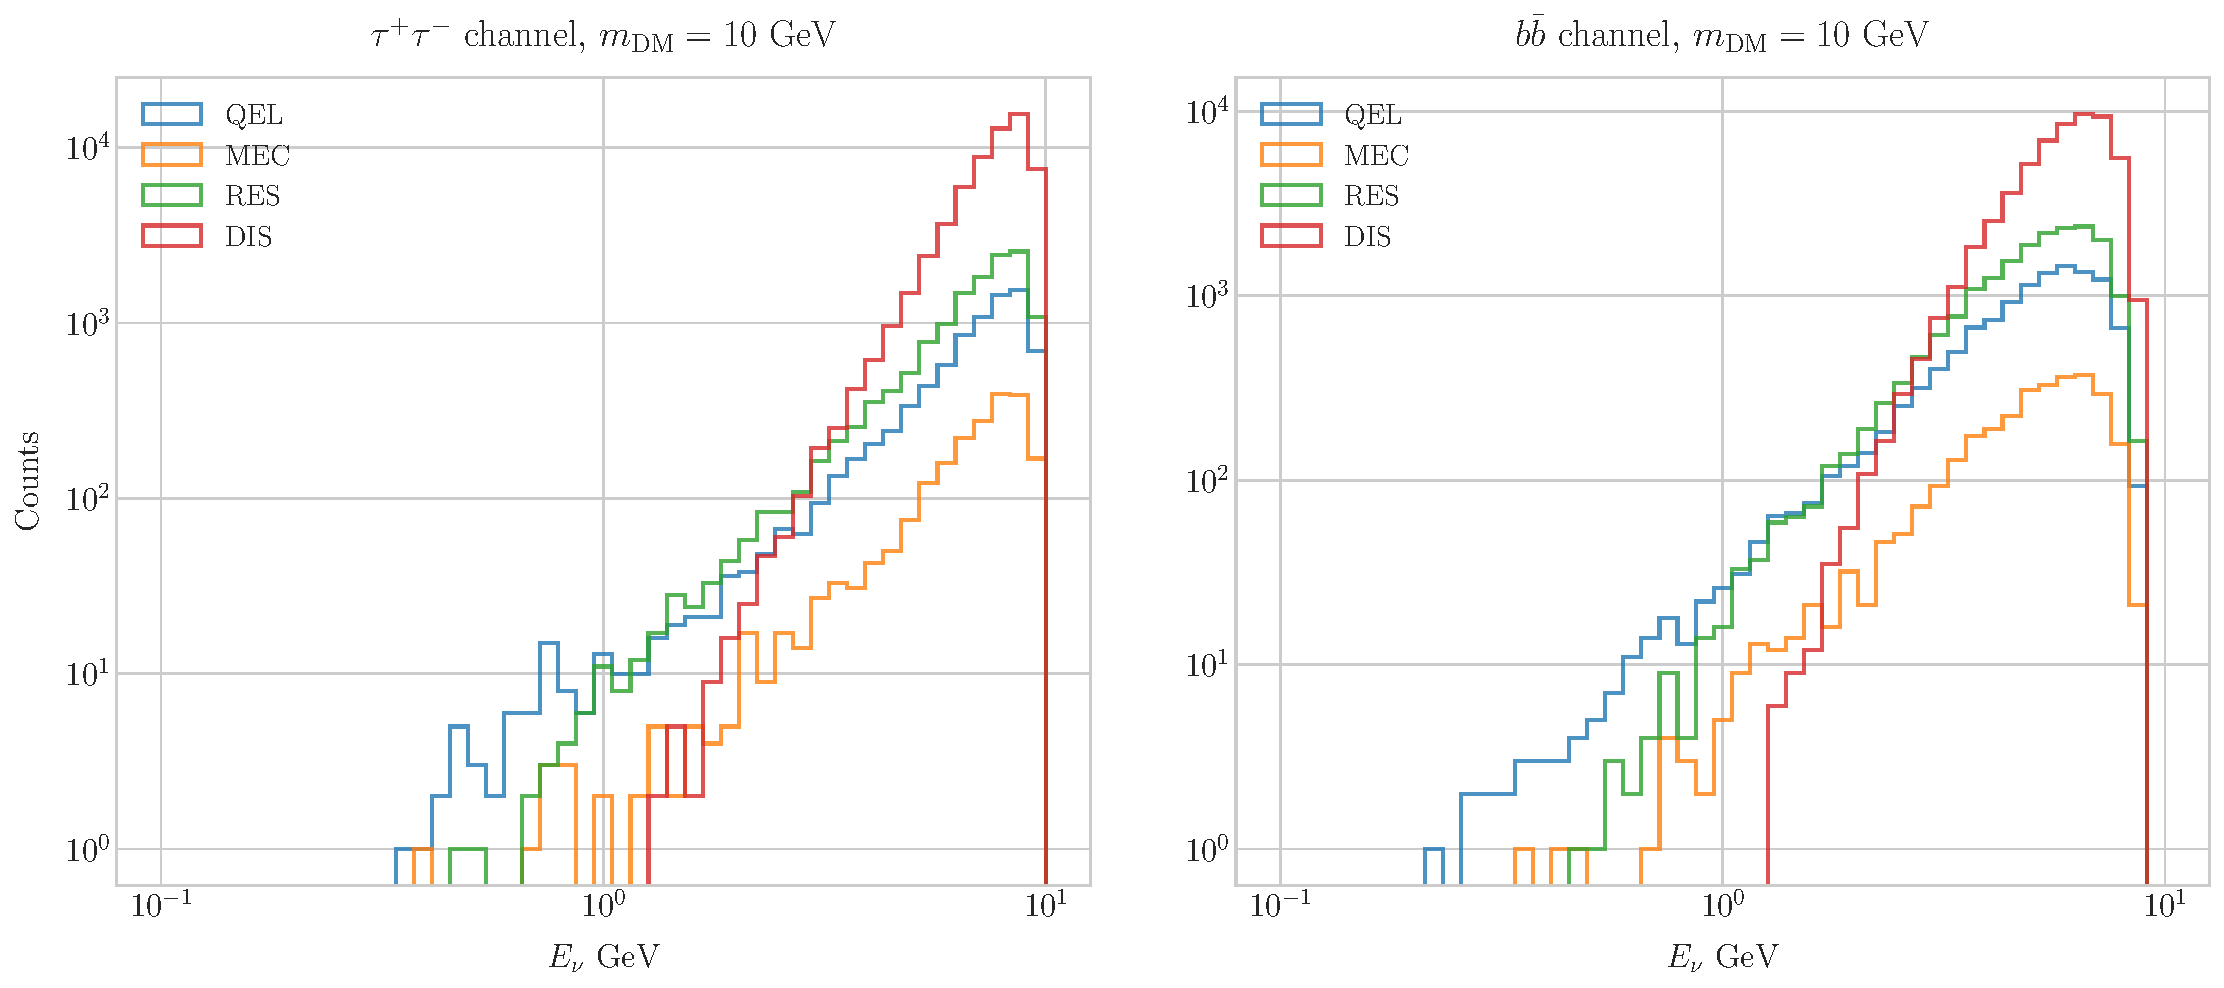
\includegraphics[width=1\linewidth]{Images/DM_Analysis/solardm_nu_mu_interactions.pdf}
	\caption[Distribution of the muon neutrino energies from the $\tau^{+} \tau^{-}$ and $b\bar{b}$ annihilation channels.]{Distribution of the muon neutrino energies from the $\tau^{+} \tau^{-}$ (left panel) and $b\bar{b}$ (right panel) annihilation channels, for $m_{\mathrm{DM}} = 10 \ \mathrm{GeV}$, separated by CC interaction type: QE (blue), MEC (orange), RES (green) and DIS (red).}
	\label{fig:solardm_nu_mu_interactions}
\end{figure}

For the atmospheric fluxes I follow a similar procedure, only that this time I do not have a set of events but the fluxes binned in azimuth and altitude angles. This way, I transform these to DUNE coordinates and process the fluxes for each bin separated with \texttt{NuWro}.

At this point, I have two sets of events with different energies and final states. In Fig. \ref{fig:solardm_nu_mu_interactions} one can see the distribution of the muon neutrino energies for the case $m_{\mathrm{DM}} = 10 \ \mathrm{GeV}$, both for the $\tau^{+} \tau^{-}$ (left panel) and $b\bar{b}$ (right panel) channels, separated by interaction. One can clearly see that there are different energy regimes where the primary interaction type is different. This leads to a plurality of event topologies, therefore making it difficult to implement a general approach to the selection of events in detriment of the background. As a way to proceed, I decided to focus on a subset of the samples, based on the different interaction modes and contents of the final state. Thus, I consider a CC DIS sample and a single proton CC QE sample.

\begin{figure}[t]
	\centering
	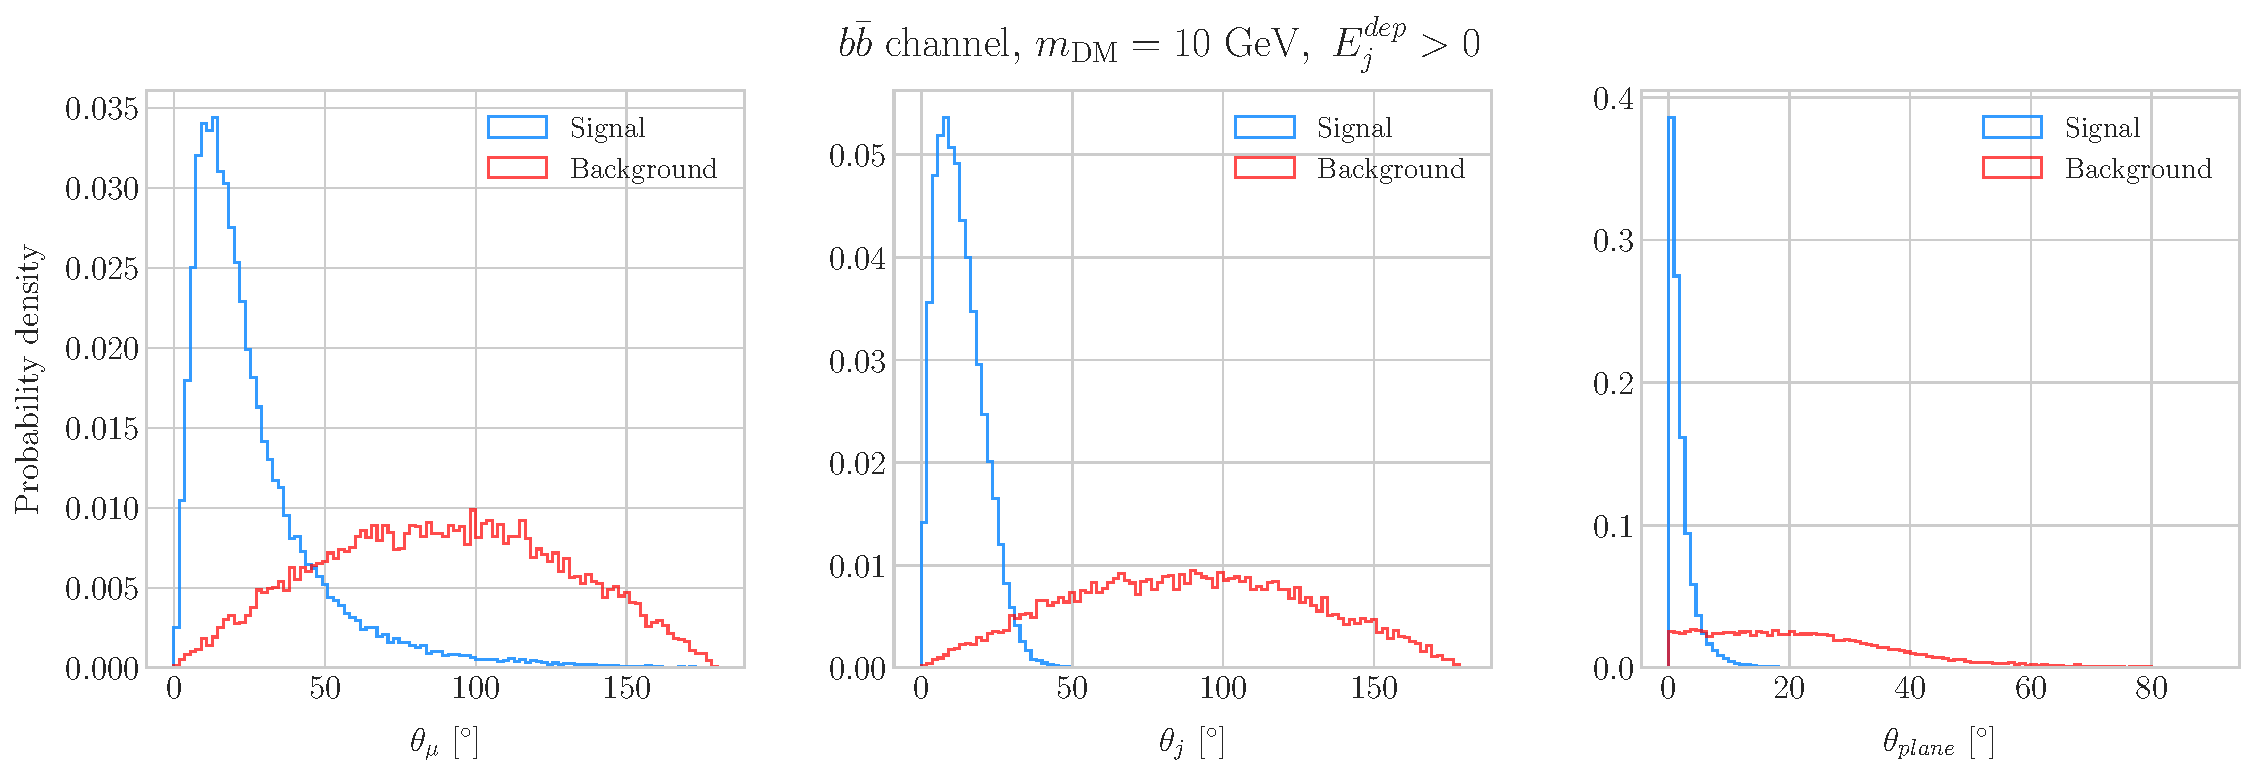
\includegraphics[width=0.95\linewidth]{Images/DM_Analysis/solardm_bb_100_dis_angular_dists.pdf}
	\caption[Angular distributions for the $b\bar{b}$ DIS sample with $m_{\mathrm{DM}} = 10 \ \mathrm{GeV}$ and the atmospheric background.]{Distributions of $\theta_{\mu}$ (left panel), $\theta_{j}$ (central panel) and $\theta_{plane}$ (right panel) for the $b\bar{b}$ sample with $m_{\mathrm{DM}} = 10 \ \mathrm{GeV}$ (blue) and the atmospheric background (red).}
	\label{fig:solardm_bb_100_dis_angular_dists}
\end{figure}

\subsection{DIS-like events}

To begin with, I consider the high energy part of the spectrum. In this region DIS events dominate, i.e. interactions of the form $\nu_{\mu} + q_{d}(\bar{q}_{u}) \rightarrow \mu^{-} + q_{u}(\bar{q}_{d})$. Therefore, our final estates will contain a muon and a hadronic jet from the fragmentation of the outgoing quark. As all these events have $E_{\nu} \gtrsim 1 \ \mathrm{GeV}$ the momentum transfer to the remnant nucleus is negligible, for this reason the neutrino energy can be effectively reconstructed just taking into account the momenta of the muon and the jet. This technique was successfully used in Ref. \cite{Rott2019} to select monoenergetic DM solar neutrino events from $\nu \bar{\nu}$ annihilation channels.

Using momentum conservation one sees that the plane generated by the momenta of the muon and the jet needs to also contain the momentum of the neutrino. As we are interested in neutrinos coming from the Sun, the momentum of the neutrino can be regarded as known beforehand. This will allow us to define the angle of the outgoing muon and jet with respect to the incoming neutrino. Moreover, one can also use that information to reject poorly reconstructed jets, checking for deviations of these from the momentum conservation plane.

To account for the limited angular resolution of the detector, I smeared the momenta of the muons and hadrons. In a LArTPC muons are expected to be tracked with high precision, therefore I take the associated angular resolution to be $1^{\circ}$. In the case of jets, it is expected that for the hadrons dominating the cascade a detector like DUNE has an angular resolution between $1^{\circ}$ to $5^{\circ}$ \cite{DUNE2020TDR2}, so I take the latter, more conservative, estimate.

As a first selection step, I will just take into account particles with kinetic energies above the detection threshold of DUNE. For muons and photons the specified threshold energy is $30 \ \mathrm{MeV}$, for charged pions $100 \ \mathrm{MeV}$ and for other hadrons $50 \ \mathrm{MeV}$ \cite{DUNE2020TDR2}. This way, if the outgoing muon in a certain event has an energy lower than the required threshold I will drop such event. For the case of hadrons and photons, I will only require to have at least one particle above the energy threshold, so then one can compute the jet momentum using the (smeared) momenta of the $N$ particles above threshold as:
\begin{equation}
	\vec{p}_{j} = \sum_{i=1}^{N} \vec{p}_{i}.
\end{equation}

\begin{figure}[t]
	\centering
	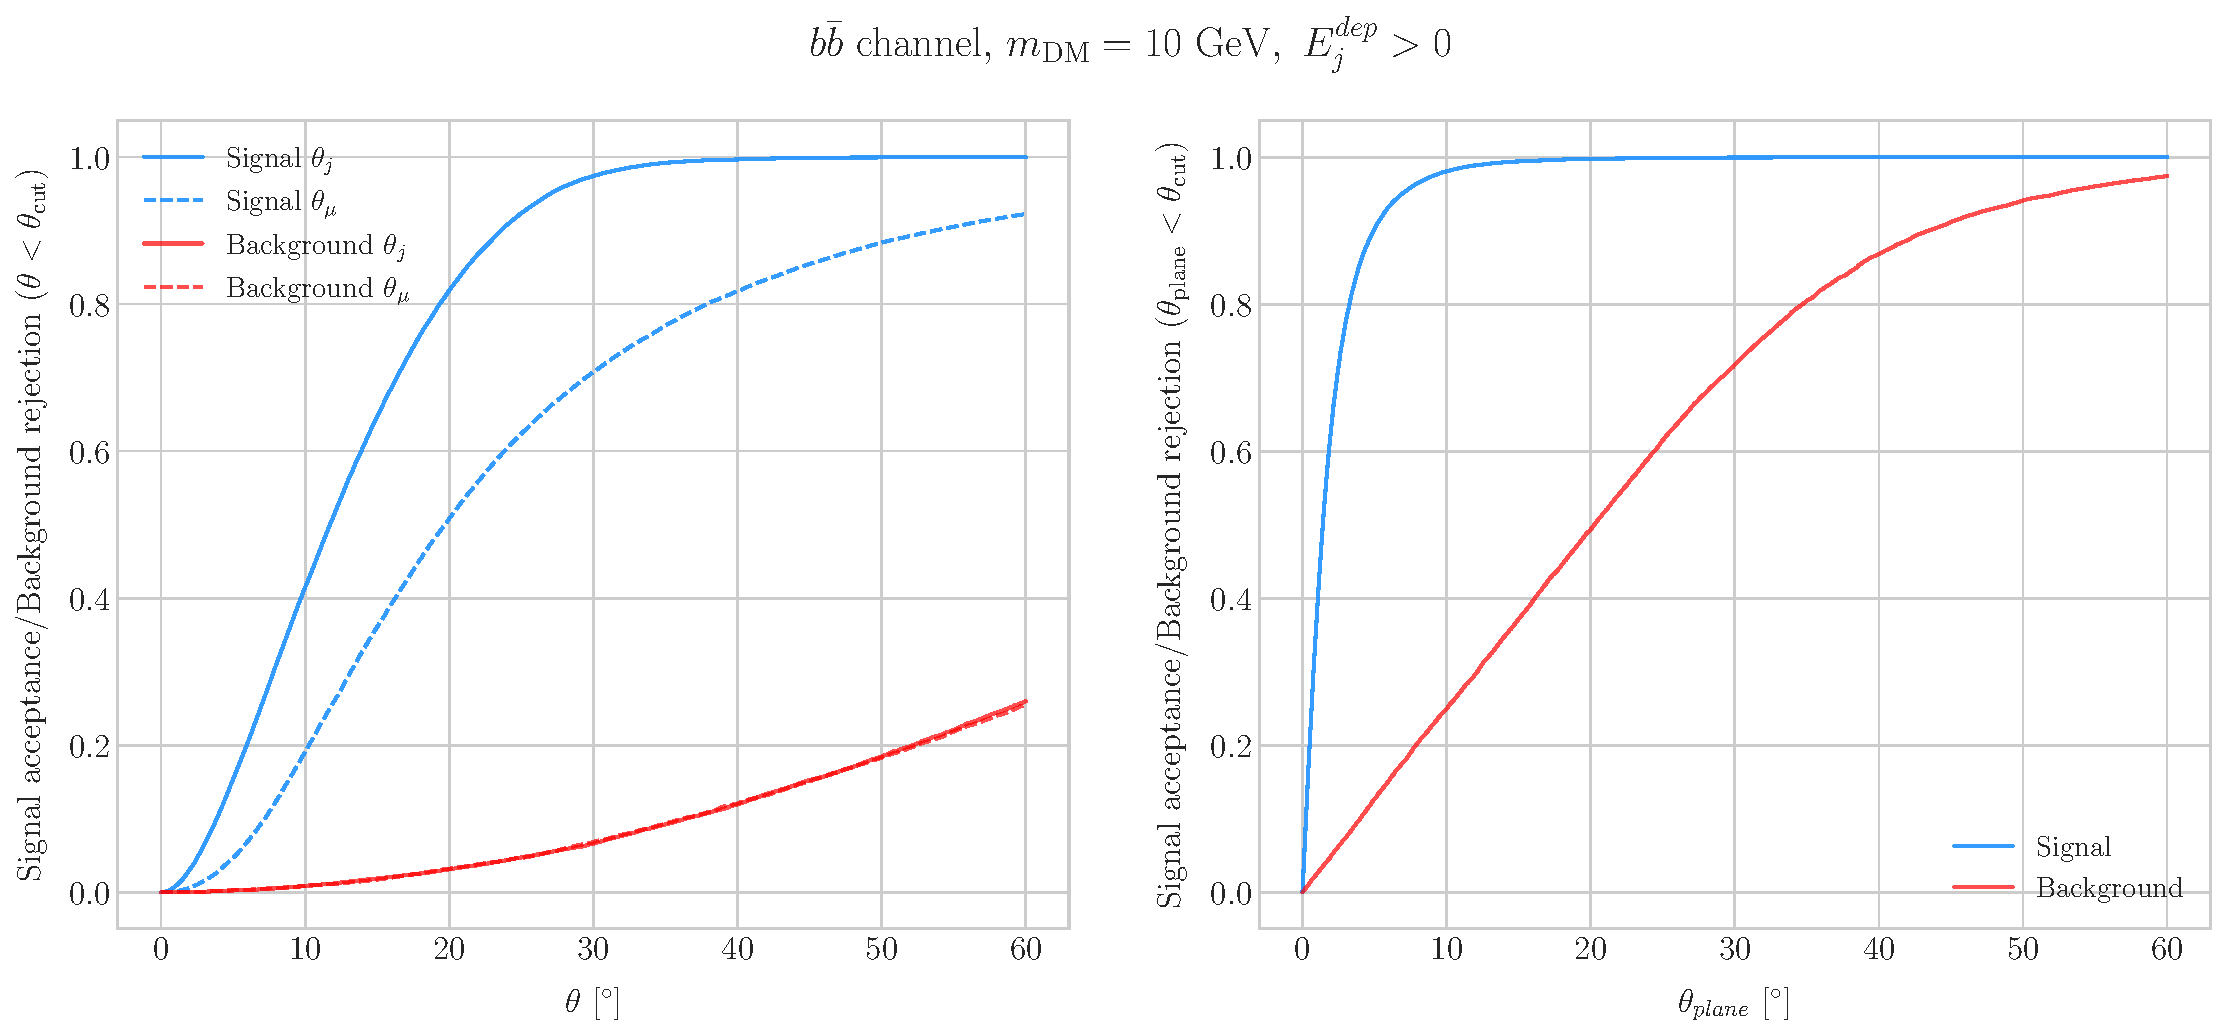
\includegraphics[width=0.95\linewidth]{Images/DM_Analysis/solardm_bb_100_dis_angular_cuts.pdf}
	\caption[Signal efficiency and background rejection for the $b\bar{b}$ sample with $m_{\mathrm{DM}} = 10 \ \mathrm{GeV}$ as a function of the angular cuts.]{Left panel: signal efficiencies (blue lines) and background rejections (red lines) for events passing the cuts $\theta < \theta_{cut}$ for the jet (solid lines) and muon (dashed lines) angles. Right panel: signal efficiency (blue line) and background rejection (red line) for events passing the cut $\theta_{plane} < \theta_{cut}$ for the momentum conservation plane deviation.}
	\label{fig:solardm_bb_100_dis_angular_cuts}
\end{figure}

Additionally, I will also define an estimation of the deposited hadronic energy as:
\begin{equation}
	E_{j}^{dep} = m_{^{39}\mathrm{Ar}} - m_{^{40}\mathrm{Ar}} + \sum_{i=1}^{N} \sqrt{|\vec{p}_{i}|^{2} + m_{i}^{2}}.
\end{equation}
This quantity is useful to select events with enough hadronic visible energy in the detector. For events where most of the hadronic energy is scattered across plenty of hadrons with individual energies below the detection threshold, this estimation will give $E_{j}^{dep} \leq 0$. In these cases it could be expected that the jet momentum is poorly reconstructed, and therefore I require events to pass the cut $E_{j}^{dep} > 0$.

For the events I can compute the angles for the muon and jet with respect to the incoming neutrino as:
\begin{align}
	\mathrm{cos} \ \theta_{\mu} &= \hat{p}_{\nu} \cdot \hat{p}_{\mu},\\
	\mathrm{cos} \ \theta_{j} &= \hat{p}_{\nu} \cdot \hat{p}_{j},
\end{align}
and the deviation from the momentum conservation plane as:
\begin{equation}
	\mathrm{sin} \ \theta_{plane} = \left|\frac{\hat{p}_{\mu} \cross \hat{p}_{\nu}}{|\hat{p}_{\mu} \cross \hat{p}_{\nu}|} \cdot \hat{p}_{j}\right|.
\end{equation}

In Fig. \ref{fig:solardm_bb_100_dis_angular_dists} I show some distributions of these quantities for the case of the $b\bar{b}$ sample with $m_{\mathrm{DM}} = 10 \ \mathrm{GeV}$ (blue histograms) and for the atmospheric backgrounds (red). In order to select the atmospheric events I followed the same criteria as for the signal events. However, because in the signal case I used the true direction of the neutrino as input, as it should be that of the Sun at that time and therefore known, in the atmospheric case I used a set of solar positions as our ansatz for the neutrino direction. From the distributions, one can see that the muon and the jet for the signal events are predominantly forward and also that the deviations from the momentum conservation plane are peaked at zero, as one should expect.

\begin{figure}[t]
	\centering
	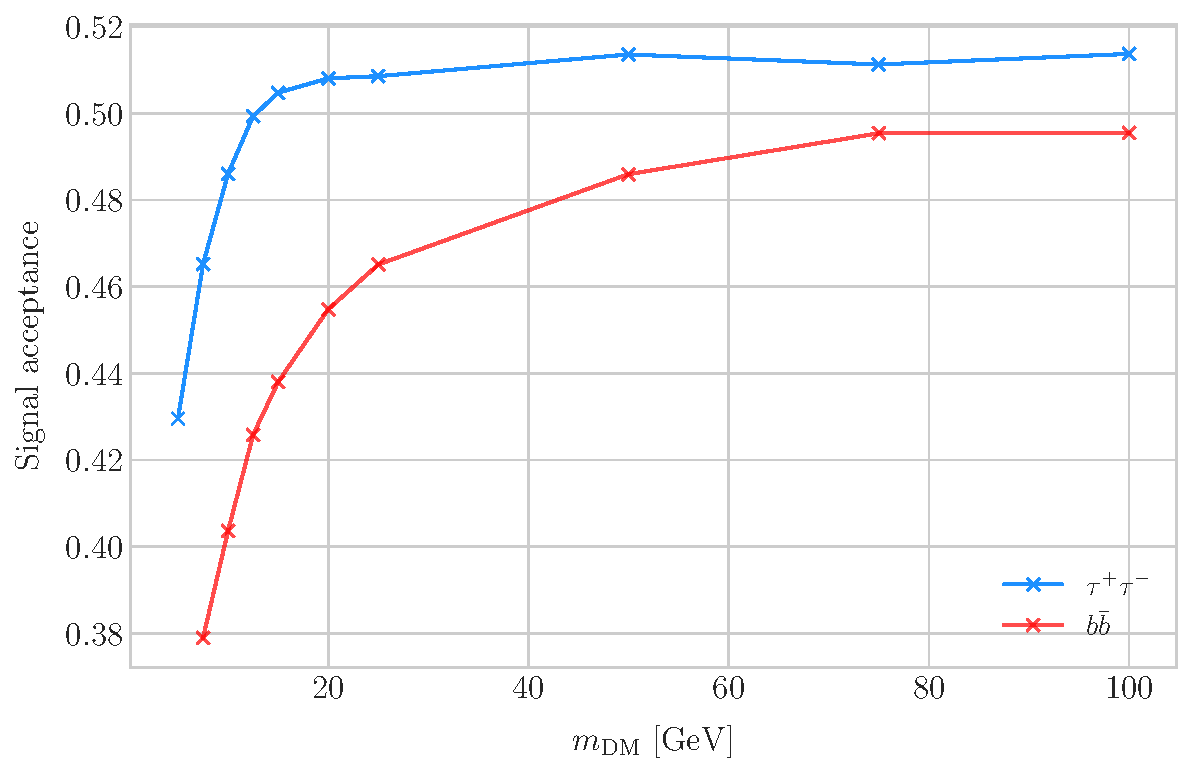
\includegraphics[width=0.9\linewidth]{Images/DM_Analysis/solardm_dis_signal_acceptance.pdf}
	\caption[Signal efficiencies for the $\tau^{+} \tau^{-}$ and $b\bar{b}$ DIS samples as functions of the DM mass.]{Signal efficiencies for the $\tau^{+} \tau^{-}$ (blue line) and $b\bar{b}$ (red line) DIS samples as functions of the DM mass, $m_{\mathrm{DM}}$, obtained by applying the optimal angular cuts $\theta_{\mu} < 27^{\circ}$, $4^{\circ} < \theta_{j} < 26^{\circ}$ and $\theta_{plane} < 3.5^{\circ}$.}
	\label{fig:solardm_dis_efficiency}
\end{figure}

Now, I can start applying cuts to maximise our signal selection efficiency while at the same time I try to minimise the amount of atmospheric background events passing the selection. To this end, I will need at to find some lower and upper cuts for $\theta_{j}$ and $\theta_{\mu}$ and an upper bound for $\theta_{plane}$. In Fig. \ref{fig:solardm_bb_100_dis_angular_cuts} I show how upper bound cuts in the different angular variables affect the signal efficiency (blue lines) and the background rejection (red lines). Notice that the signal efficiency behaves in a quite different way when I apply cuts in the jet and the muon angles. On the contrary, the cuts on both variables have a similar effect on the background rejection.

In order to obtain the optimal set of cuts, I perform a multidimensional scan. I do this separately for the $\tau^{+} \tau^{-}$ and the $b\bar{b}$ samples. For each case, I scan the possible cuts for each mass point and then I take the mean value of the signal efficiency for each configuration, to get the mean efficiency for each set of cuts. I do a similar scan for the atmospheric sample independently. Then, I take the sets of cuts such that the background rejection achieved is greater than $99.8\%$ and search for the one which maximises the $\tau^{+} \tau^{-}$ and $b\bar{b}$ sample mean efficiencies. I found that with the cuts $\theta_{\mu} < 27^{\circ}$, $4^{\circ} < \theta_{j} < 26^{\circ}$ and $\theta_{plane} < 3.5^{\circ}$ I get a background rejection of $99.80\%$ while achieving a $49.40\%$ and $44.92\%$ mean signal efficiencies for the $\tau^{+} \tau^{-}$ and $b\bar{b}$ signals respectively.

In Fig. \ref{fig:solardm_dis_efficiency} I show the signal efficiencies as a function of the DM mass for the $\tau^{+} \tau^{-}$ (blue line) and the $b\bar{b}$ (red line) DIS events, after applying the cuts discussed above, as well as the energy threshold and hadronic visible energy selections. One can see that the efficiency grows with the mass, as annihilations of more massive DM particles will produce a neutrino spectrum centered at higher energies, where DIS events dominate. Notice also that the efficiency is higher for the $\tau^{+} \tau^{-}$ case at every mass point, as in general this channel produces neutrinos at higher energies than the corresponding $b\bar{b}$ channel.

\begin{figure}[t]
	\centering
	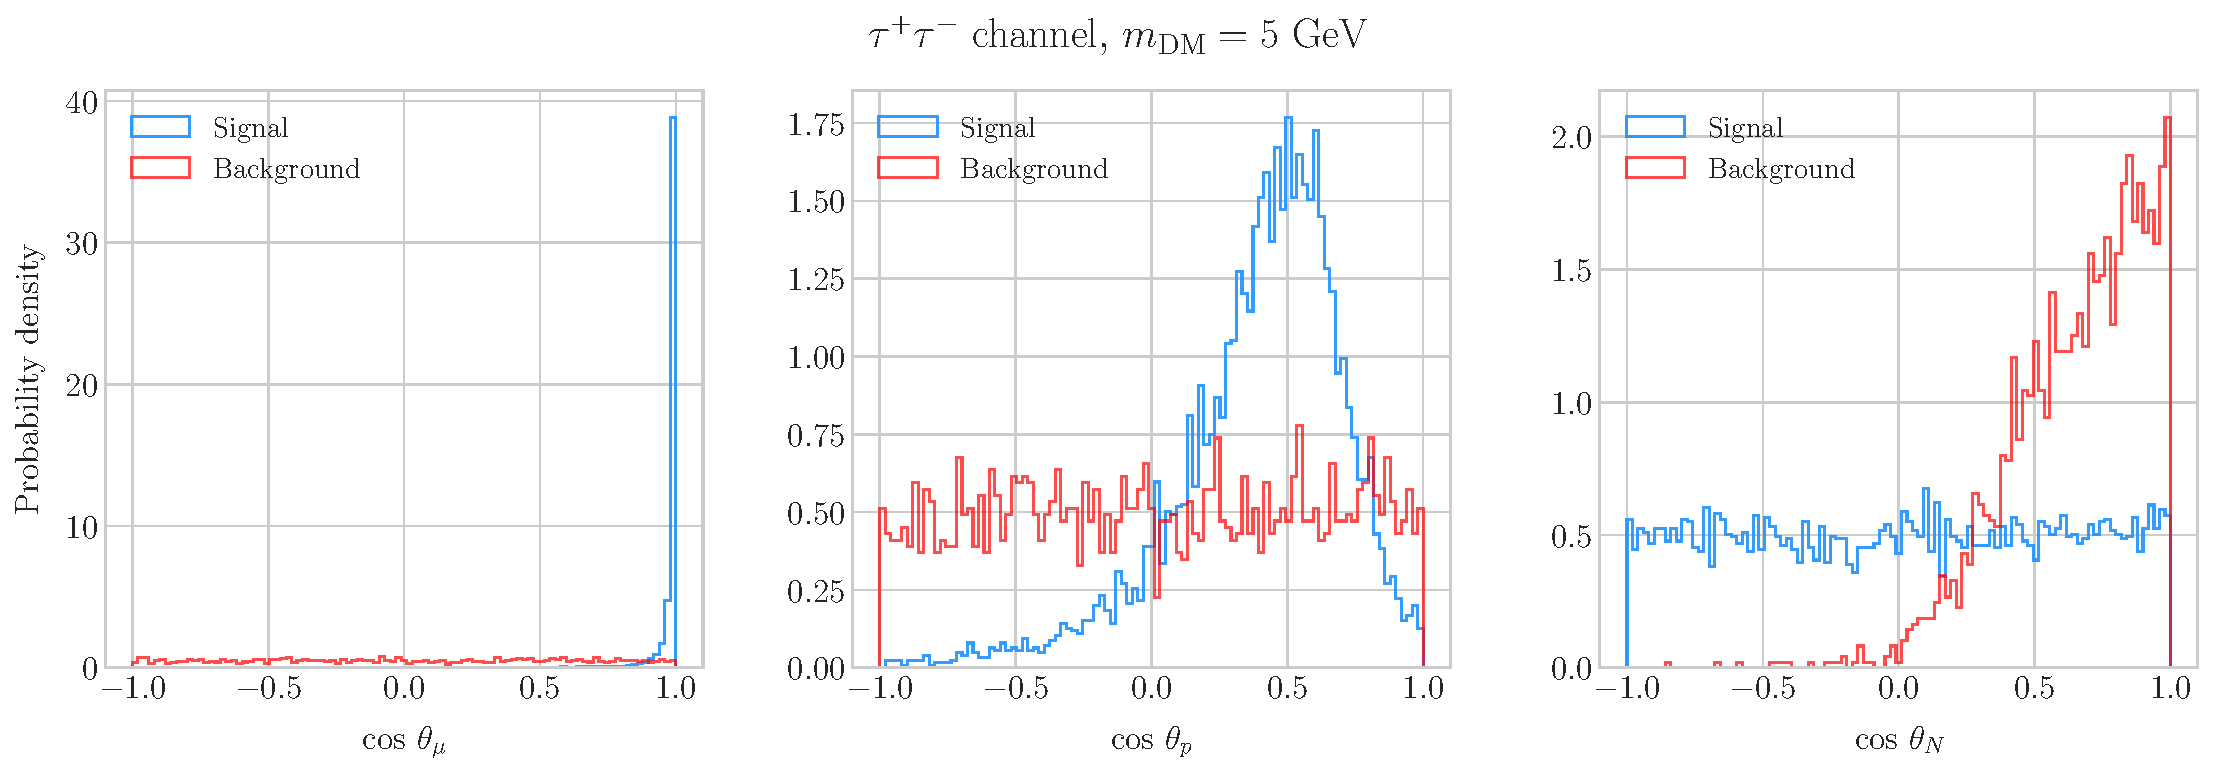
\includegraphics[width=0.95\linewidth]{Images/DM_Analysis/solardm_tau_5_qel_angular_dists.pdf}
	\caption[Angular distributions for the $\tau^{+}\tau^{-}$ QE sample with $m_{\mathrm{DM}} = 5 \ \mathrm{GeV}$ and the atmospheric background.]{Distributions of $\mathrm{cos} \ \theta_{\mu}$ (left panel), $\mathrm{cos} \ \theta_{p}$ (central panel) and $\mathrm{cos} \ \theta_{N}$ (right panel) for the $\tau^{+}\tau^{-}$ QE sample with $m_{\mathrm{DM}} = 5 \ \mathrm{GeV}$ (blue) and the atmospheric background (red).}
	\label{fig:solardm_tau_5_qel_angular_dists}
\end{figure}

\subsection{Single proton QE-like events}

Now, one can try to explore the low energy tail of the neutrino energy distributions. This regime is dominated by the QE interactions, i.e. events of the type $\nu_{\mu} + n \rightarrow \mu^{-} + p$. In this case, as the typical energies are $E_{\nu} \lesssim 1 \ \mathrm{GeV}$, the momentum transfer to the remnant nucleus is sizeable. Therefore, I can not make the approximation I did before and assume that the momentum of the muon and the proton will give an adequate estimation of the reconstructed neutrino energy.

In any case, as before, I can take the direction of the incoming neutrino as known. That way, one can estimate the energy of the neutrino as:
\begin{equation}\label{6.6}
	E_{\nu}^{reco} = E_{\mu} + E_{p} + m_{^{39}\mathrm{Ar}} - m_{^{40}\mathrm{Ar}},
\end{equation}
and using momentum conservation I can write the momentum of the remnant nucleus as:
\begin{equation}\label{6.7}
	\vec{p}_{N} = \hat{p}_{\nu} \left(E_{\mu} + E_{p} + m_{^{39}\mathrm{Ar}} - m_{^{40}\mathrm{Ar}}\right) - \vec{p}_{\mu} - \vec{p}_{p}.
\end{equation}

As in the previous case, I need to drop the events where the muon or the proton fall below the kinetic energy detection threshold \cite{DUNE2020TDR2}. Also, I again apply a smearing to the momenta of the particles, a $1\%$ for muons and $5\%$ for protons.

\begin{figure}[t]
	\centering
	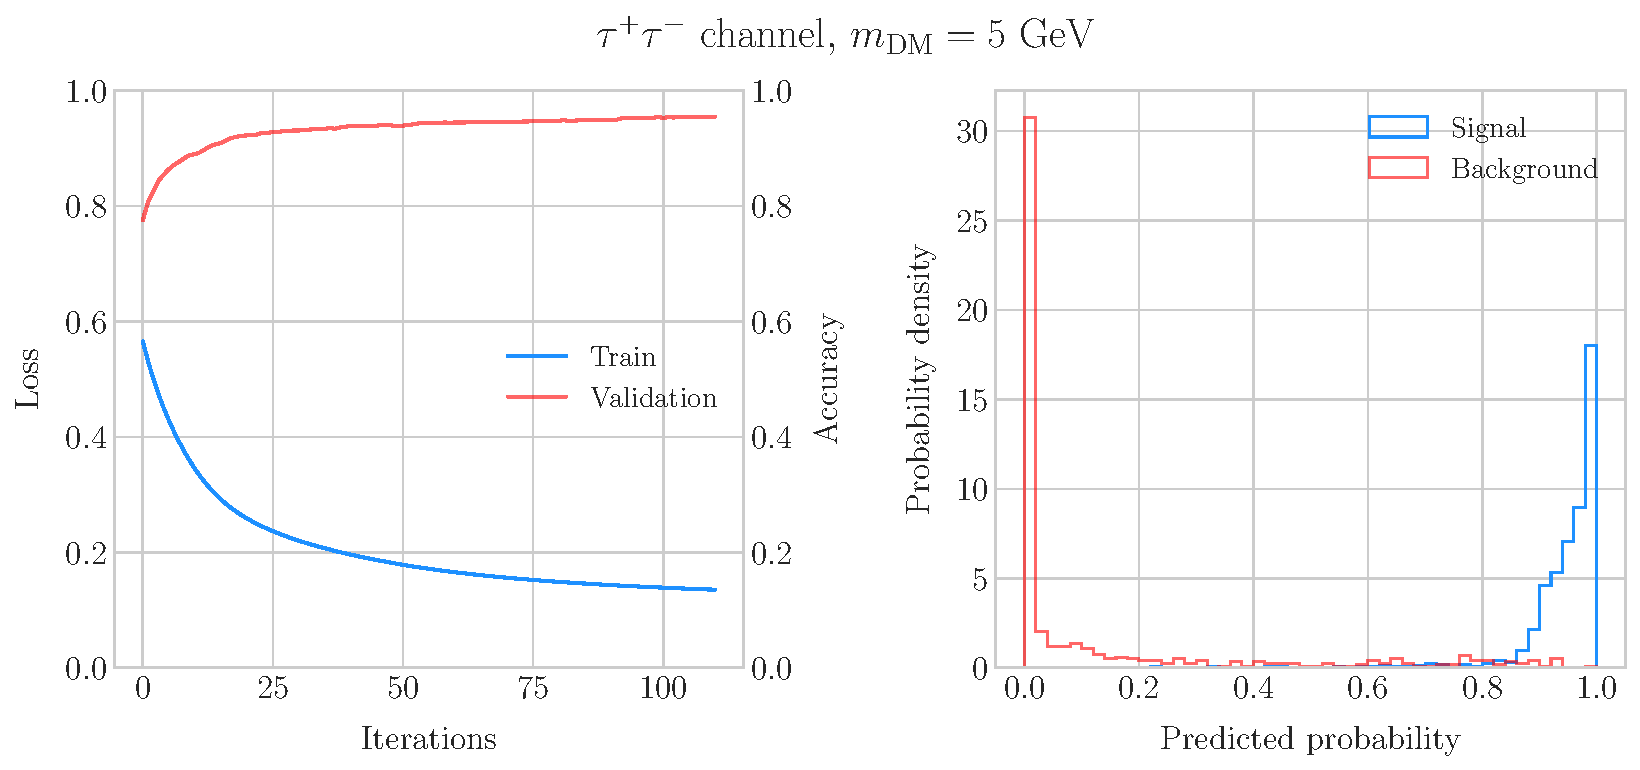
\includegraphics[width=0.95\linewidth]{Images/DM_Analysis/solardm_tau_5_qel_classifier.pdf}
	\caption[Performance of the MLP classifier for the $\tau^{+}\tau^{-}$ QE signal with $m_{\mathrm{DM}} = 5 \ \mathrm{GeV}$.]{Left panel: value of the loss function for the training sample (blue line) and accuracy for the validation sample (red line) versus the number of iterations for the MLP classifier training. Right panel: distributions of the predicted probabilities assigned by the MLP classifier to the test sample for the $\tau^{+}\tau^{-}$ QE signal with $m_{\mathrm{DM}} = 5 \ \mathrm{GeV}$ (blue) and the atmospheric background (red).}
	\label{fig:solardm_tau_5_qel_classifier}
\end{figure}

Having done that, one can compute the following angular variables for our selected events:
\begin{align}
	\mathrm{cos} \ \theta_{\mu} &= \hat{p}_{\nu} \cdot \hat{p}_{\mu},\label{6.8} \\
	\mathrm{cos} \ \theta_{p} &= \hat{p}_{\nu} \cdot \hat{p}_{p},\label{6.9} \\
	\mathrm{cos} \ \theta_{N} &= \hat{p}_{\nu} \cdot \hat{p}_{N}. \label{6.10}
\end{align}

Fig. \ref{fig:solardm_tau_5_qel_angular_dists} shows the distributions of these angular variables for the $\tau^{+}\tau^{-}$ QE sample with $m_{\mathrm{DM}} = 5 \ \mathrm{GeV}$ (blue) and the atmospheric background (red). Again, for the atmospheric events I used a random solar position as the ansatz for the incoming neutrino direction. Notice that now, opposed to the DIS case where the signal had very sharp distributions for the variables considered, the shapes of the angular distributions for signal and background are not that much different.

This effectively means that the usual approach of applying simple angular cuts would not work as well as in the previous situation. Therefore, as a possible solution, I tried to use a multilayer perceptron (MLP) classifier to separate between signal and background events. Thus, the power of the hypothesis test will serve as an estimate of the signal efficiency, and in the same way one can take the size of the test to be our background rejection.

For each DM mass value and channel, as well as for the background sample, I divide our events into training, validation and test samples. The input variables for the classifier were the reconstructed neutrino energy from Eq. (\ref{6.6}) and the angular variables defined in Eqs. (\ref{6.8} - \ref{6.10}). I used the MLP classifier implemented in \texttt{scikit-learn} \cite{scikit-learn}, with a total of five hidden layers, the rectified linear unit activation function and adaptive learning rate. In order to account for fluctuations due to artifacts in the training process I repeated the training a thousand times for each sample, redefining each time the training, validation and test subsets, so one can take as our signal efficiency and background rejection the mean values of the powers and sizes of the tests.

\begin{figure}[t]
	\centering
	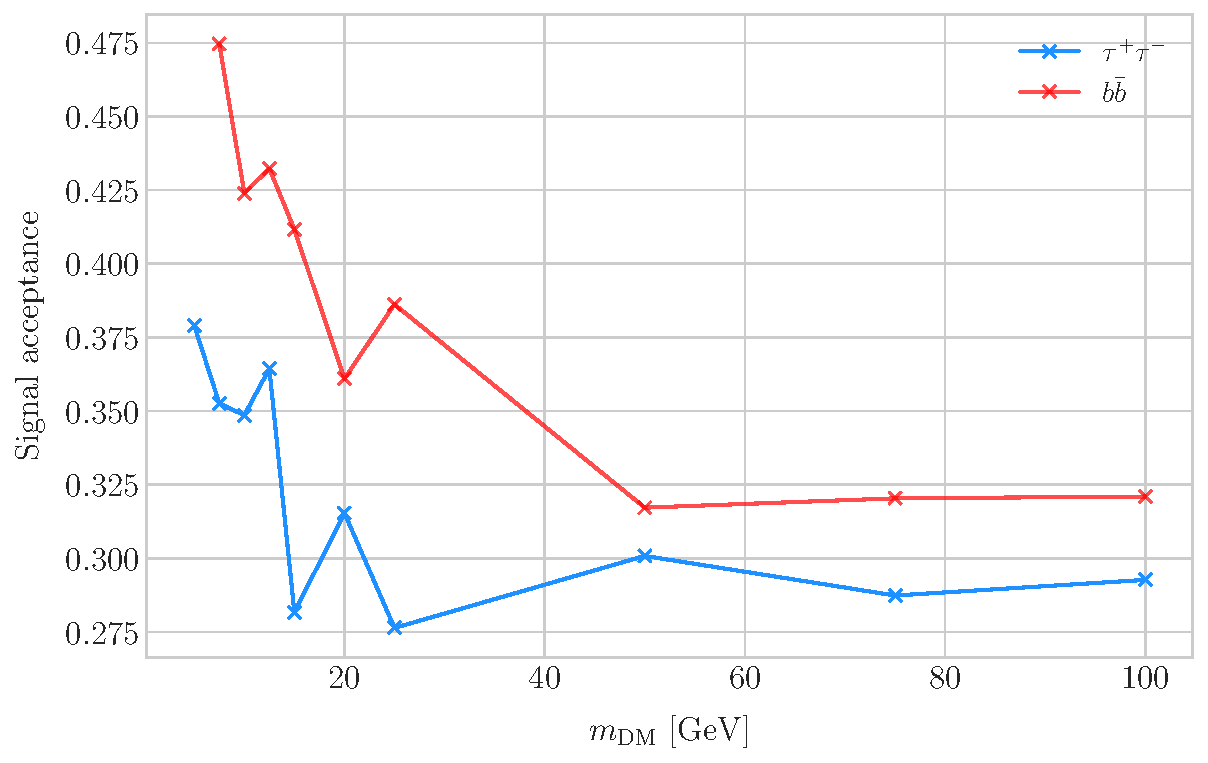
\includegraphics[width=0.9\linewidth]{Images/DM_Analysis/solardm_qel_signal_acceptance.pdf}
	\caption[Signal efficiencies for the $\tau^{+} \tau^{-}$ and $b\bar{b}$ single proton QE samples as functions of the DM mass.]{Signal efficiencies for the $\tau^{+} \tau^{-}$ (blue line) and $b\bar{b}$ (red line) single proton QE samples as functions of the DM mass, $m_{\mathrm{DM}}$, obtained by requiring a minimum predicted probability from the MLP classifier of $0.97$ in order to achieve a background rejection greater than $99.8\%$.}
	\label{fig:solardm_qel_signal_acceptance}
\end{figure}

The results of one of these training processes for the $\tau^{+}\tau^{-}$ QE signal with $m_{\mathrm{DM}} = 5 \ \mathrm{GeV}$ is shown in Fig. \ref{fig:solardm_tau_5_qel_classifier}. On the left panel I show the loss function values (blue) and accuracy (red) at each iteration for the training and the validation samples respectively. The training stops either when the maximum number of iterations is reached (1000 in this case) or when the accuracy for the validation sample reaches a certain tolerance (I chose $10^{-4}$ as our tolerance). On the right panel I have the distributions for the predicted probability by the model, separated in true signal (blue) and background (red) events, for the test sample. One can see that both populations are well separated, obtaining a power of $44.97\%$ and a size of $0.17\%$ when I require a predicted probability greater than $0.97$.

Applying this criteria for each sample, I obtain the mean signal efficiencies shown in Fig. \ref{fig:solardm_qel_signal_acceptance}. Notice that the efficiencies for the  channel $\tau^{+}\tau^{-}$ (blue line) are consistently lower than the ones for the $b\bar{b}$ channel (red line). This can be due to the fact that, for each DM mass point, the neutrino spectrum coming from the $b\bar{b}$ annihilation channel is centered at lower energies when compared to the $\tau^{+}\tau^{-}$ spectrum. This directly translates into more low energy neutrinos undergoing QE interactions, which give signals that can be easily separated from the atmospheric background. This explanation also help us understand why in both cases the signal acceptance drops when the DM mass increases. In all cases, the background rejection took values between $99.8\%$ to $99.9\%$. I will assume a $99.8\%$ background rejection value in all cases to keep our estimation conservative.

\begin{figure}[t]
	\centering
	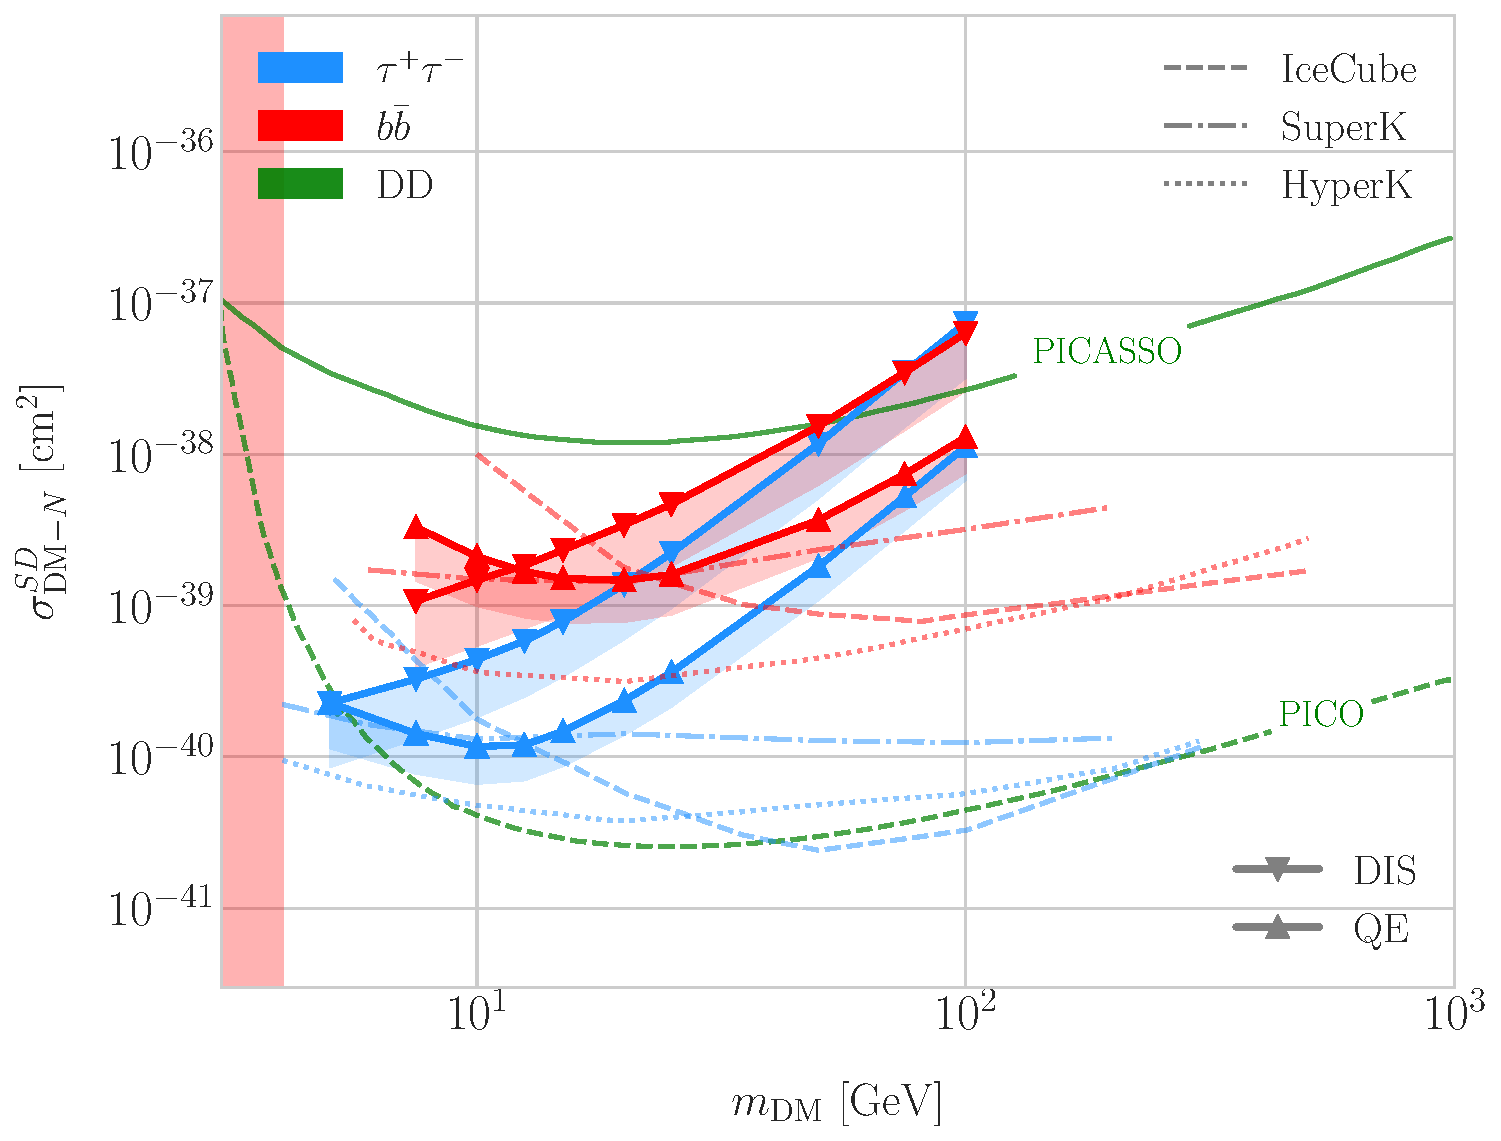
\includegraphics[width=0.95\linewidth]{Images/DM_Analysis/solardm_xsection_sd.pdf}
	\caption[Projected 90\% confidence level upper limit for DUNE (400 kT yr) on the spin-dependent DM-nucleon scattering cross section as a function of $m_{\mathrm{DM}}$, for the annihilation channels $\tau^{+}\tau^{-}$ and $b\bar{b}$ separated by interaction mode]{Projected 90\% confidence level upper limit for DUNE (400 kT yr) on the spin-dependent DM-nucleon scattering cross section as a function of $m_{\mathrm{DM}}$, for the annihilation channels $\tau^{+}\tau^{-}$ (blue) and $b\bar{b}$ (red) separated by interaction mode (up triangles denote DIS interactions whereas down triangles represent QE interactions). I also show the previous limits from IceCube \cite{IceCube2021} (solid lines) and the projected sensitivities for Pingu \cite{Chen2014} (dashed lines) and Hyper-Kamiokande \cite{Bell2021} (dash-dotted lines), as well as the direct detection limits from PICASSO \cite{Behnke2016} (solid green line) and PICO-60 $\mathrm{C}_{3}\mathrm{F}_{8}$ \cite{PICO2019} (dashed green line).}
	\label{fig:solardm_xsection_sd}
\end{figure}

\subsection{Results}

In order to estimate the DM-nucleon cross section sensitivities in the present case I need again to compute the expected number of background events. As I am now separating events by interaction type Eq. (\ref{4.4}) does not hold anymore, as in that case I integrated over the total neutrino-argon cross section. In this instance, the expected background events for DIS events is approximately given by:
\begin{equation}\label{6.11}
	N_{B}^{DIS} \simeq \eta_{B}^{DIS} \times \left(4.655 \times 10^{3}\right) \times \left(\frac{\mathrm{exposure}}{400 \ \mathrm{kT} \ \mathrm{yr}}\right),
\end{equation}
whereas for QE events we have:
\begin{equation}\label{6.12}
	N_{B}^{QE} \simeq \eta_{B}^{QE} \times \left(2.248\times 10^{4}\right) \times \left(\frac{\mathrm{exposure}}{400 \ \mathrm{kT} \ \mathrm{yr}}\right).
\end{equation}

Now, using these together with Eqs. (\ref{4.5}) and (\ref{4.6}) one can obtain the $90\%$ C.L. upper limit on the total annihilation rate at equilibrium for both kind of events. Then, applying the computed DM-nucleons capture rates I can translate these into limits on the DM-nucleon cross section by means of Eqs. (\ref{2.2}), (\ref{2.5}) and (\ref{2.6}).

Fig. \ref{fig:solardm_xsection_sd} shows the obtained limits on the SD DM-nucleon cross section for DUNE, using the DIS (up triangles) and QE (down triangles) events both for the $\tau^{+}\tau^{-}$ (blue) and the $b\bar{b}$ (red) samples, for an exposure of $400 \ \mathrm{kT} \ \mathrm{yr}$. I also include the corresponding current limits from IceCube \cite{IceCube2021} (solid lines), as well as the projected sensitivities of Pingu \cite{Chen2014} (dashed lines) and Hyper-Kamiokande \cite{Bell2021} (dash-dotted lines). For comparison, I also show the reported direct detection limits from PICASSO \cite{Behnke2016} (solid green line) and PICO-60 $\mathrm{C}_{3}\mathrm{F}_{8}$ \cite{PICO2019} (dashed green line).

Notice that, for most of the mass range, the limits one can set by using the DIS events are stronger than those of the QE interactions, except for the low mass part of both the $\tau^{+}\tau^{-}$ and the $b\bar{b}$ curves where the QE events dominate. In general, the expected sensitivity of DUNE for DM masses $\lesssim 25 \ \mathrm{GeV}$ surpasses the stronger current indirect limits. However, experiments like Hyper-Kamiokande are foreseen to have an overall better sensitivity in this kind of searches, as they have a bigger active volume and accept a broader energy range.

A pending question is what happens when we add the RES and MEC charged-current interaction contributions. In that case it would probably be more convenient to split the samples by final state interaction topologies. Also, another necessary improvement would be adding a full detector simulation and reconstructions. This will also require considering the effect of poorly reconstructed events or final states containing neutral particles such that they mimic the desired topology at the reconstruction level.

\begin{comment}
	In Apps. \ref{sec:B.2} and \ref{sec:B.3} I show the results of two additional studies, where I apply the techniques described before to two specific realisations of the DM interactions (Kaluza-Klein DM and leptophilic DM).
\end{comment}

\section{Example: Leptophilic Dark Matter}
\label{sec:dm_analysis_leptophilic_dm}

In general, the capture rate of DM particles by the Sun via interactions with electrons is several orders of magnitude smaller than the capture via DM-nucleus scattering. Thus, it would be sub-leading even when nucleon capture is loop suppressed. As I showed in Fig. \ref{fig:capture_rates}, the capture rate via scattering off electrons only surpasses the capture rates via DM-nucleons interactions for DM masses $\lesssim 100 - 500 \ \mathrm{MeV}$.

However, if one considers a model where DM-nucleon interactions are forbidden even at loop level, then electron interactions will be the sole contributor to DM capture in the Sun. One can describe such scenario where the DM particles couple to leptons but not to the quark sector using effective operators.

In general, assuming that the DM particle is a Dirac fermion, the dimension six operators describing the interaction between two DM particles and two leptons can be written as:
\begin{equation}\label{7.1}
	\mathcal{L}_{eff} = G \sum_{i} \left(\bar{\chi} \Gamma^{i}_{\chi} \chi\right)\left(\bar{\ell} \Gamma^{i}_{\ell} \ell\right),
\end{equation}
where $G=1/\Lambda^{2}$ is the effective coupling strength, $\Lambda$ the cut-off of the effective field theory and $\ell$ denotes any lepton. In principle, one should consider all the possible Lorentz structures $\Gamma^{i}_{f}$ in order to have a complete set of effective operators.

However, some combinations will induce interactions with nucleons at loop level. As we are specifically interested in interactions which forbid any communication with the quark sector, I will not consider those \cite{Kopp2009}. In addition, some of the effective operators give rise to velocity-suppressed scattering cross sections between DM particles and leptons. I will also neglect those, as the suppression goes with the square of the DM halo velocity which in units of the speed of light is $\sim 10^{-6}$.

This way, the only Lorentz tensor structure that do not induce interactions with quarks at loop level and gives a contribution to the scattering cross section that is not velocity suppress is the axial-axial interaction. The effective Lagrangian is then given by:
\begin{equation}\label{7.2}
	\mathcal{L}_{eff} = \frac{c_{A}^{\chi} c_{A}^{\ell}}{\Lambda^{2}} \left(\bar{\chi} \gamma^{\mu}\gamma^{5} \chi\right)\left(\bar{\ell} \gamma_{\mu}\gamma^{5} \ell\right),
\end{equation}
where $c_{A}^{\chi}$ and $c_{A}^{\ell}$ are the couplings for the different species. As the DM coupling appears as a common factor for any lepton choice, I will redefine the corresponding coupling $c_{A}^{\ell}$ to absorb $c_{A}^{\chi}$. Also, for simplicity, I will assume that the couplings between the DM particles and the leptons are flavour independent, i.e. I have just two couplings, $c_{A}^{e}$ for charged leptons and $c_{A}^{\nu}$ for neutrinos.

In the case of a scalar DM particle, the lowest order effective interaction with leptons happens through a dimension five operator, generating scalar and pseudoscalar interactions. However, the former induces interactions with quarks at two loop level whereas the latter gives a velocity suppressed scattering cross section.

From the effective Lagrangian in Eq. (\ref{7.2}) it can be shown that the axial-axial contribution to the scattering cross section for the fermionic DM and a charged lepton is given by:
\begin{equation}\label{7.3}
	\sigma_{\mathrm{DM}-e}^{AA} = 3 \left(c_{A}^{e}\right)^{2} \frac{m_{e}^{2}}{\pi \Lambda^{4}}.
\end{equation}

If the DM interacts exclusively with fermions, then the only annihilation channels that will give us a measurable neutrino flux coming out of the Sun are $\tau^{+}\tau^{-}$ and $\nu\bar{\nu}$. The former channel, already explored previously in the more mainstream scenario of the DM capture via scattering off nucleons, is open only for $m_{\mathrm{DM}} > m_{\tau} \simeq 1776.86 \pm 0.12 \ \mathrm{MeV}$ \cite{ParticleDataGroup2020}, a mass region where the solar DM capture by electrons is at least one order of magnitude smaller than the capture via interactions with nucleons. On the contrary, the latter allows us to explore a region where the capture rate via scattering off electrons dominates over the rest.

One downside of focusing in such low mass range is that it falls bellow the usual limit of $m_{\mathrm{evap}} \sim 4 \ \mathrm{GeV}$ usually explored in the literature. The pretext to explore this region is the result discussed previously reported in Ref. \cite{Palomares2017}, where DM evaporation in the Sun for the case of capture via electron scattering could be negligible for masses as low as $m_{\mathrm{evap}} \sim 200 \ \mathrm{MeV}$. This result is quite sensitive to the high velocity tail of the DM velocity distribution in equilibrium inside the Sun, and therefore full numerical simulations would be needed to asses the impact of this effect. However, this falls out of the scope of our work.

In this case, as I have an specific realisation of the interaction between the DM and leptons, one can estimate the relic density of our DM for different values of the couplings and the effective field theory scale $\Lambda$. The first step to do so is compute the self-annihilation cross section. Because I consider cold relics, at the freeze-out time our DM particles were non-relativistic and so one can expand the annihilation cross section in terms of the relative velocity $v$ between two annihilating DM particles as \cite{Beltran2008}:
\begin{equation}\label{7.4}
	\sigma_{ann}^{AA}|v| \approx \frac{1}{2\pi\Lambda^{4}} \sum_{\ell} \left(c_{A}^{\ell}\right)^{2} m_{\chi}^{2} \sqrt{1-\frac{m_{\ell}^{2}}{m_{\chi}^{2}}} \left[\frac{m_{\ell}^{2}}{m_{\chi}^{2}}+\frac{1}{12}\left(2-\frac{m_{\ell}^{2}}{m_{\chi}^{2}}\right)v^{2}\right],
\end{equation}
where the sum includes all the possible lepton final states with mass $m_{\ell}$.

Solving the Boltzmann equation for the evolution of the DM density gives as a solution a relic density of:
\begin{equation}\label{7.5}
	\Omega_{\chi} h^{2} \approx \frac{(1.04 \times 10^{9}) x_{F}}{M_{Pl} \sqrt{g_{*}}(a+3b/x_{F})},
\end{equation}
where $x_{F} = m_{\chi}/T_{F}$ being $T_{F}$ the freeze-out temperature, $g_{*}$ the number of relativistic degrees of freedom at freeze-out and $a$ and $b$ the terms in the annihilation cross section expansion $\sigma_{ann} |v| \approx a + b v^{2} + \mathcal{O}(v^{4})$. Using the current best fit for the relic DM density $\Omega_{\chi} h^{2} = 0.1198 \pm 0.0012$ \cite{Planck2018} one can use these relations to compute the required effective theory scale $\Lambda$ at which the correct density is achieved for any combinations of $m_{\chi}$ and $c_{A}^{\ell}$.

\begin{figure}[t]
	\centering
	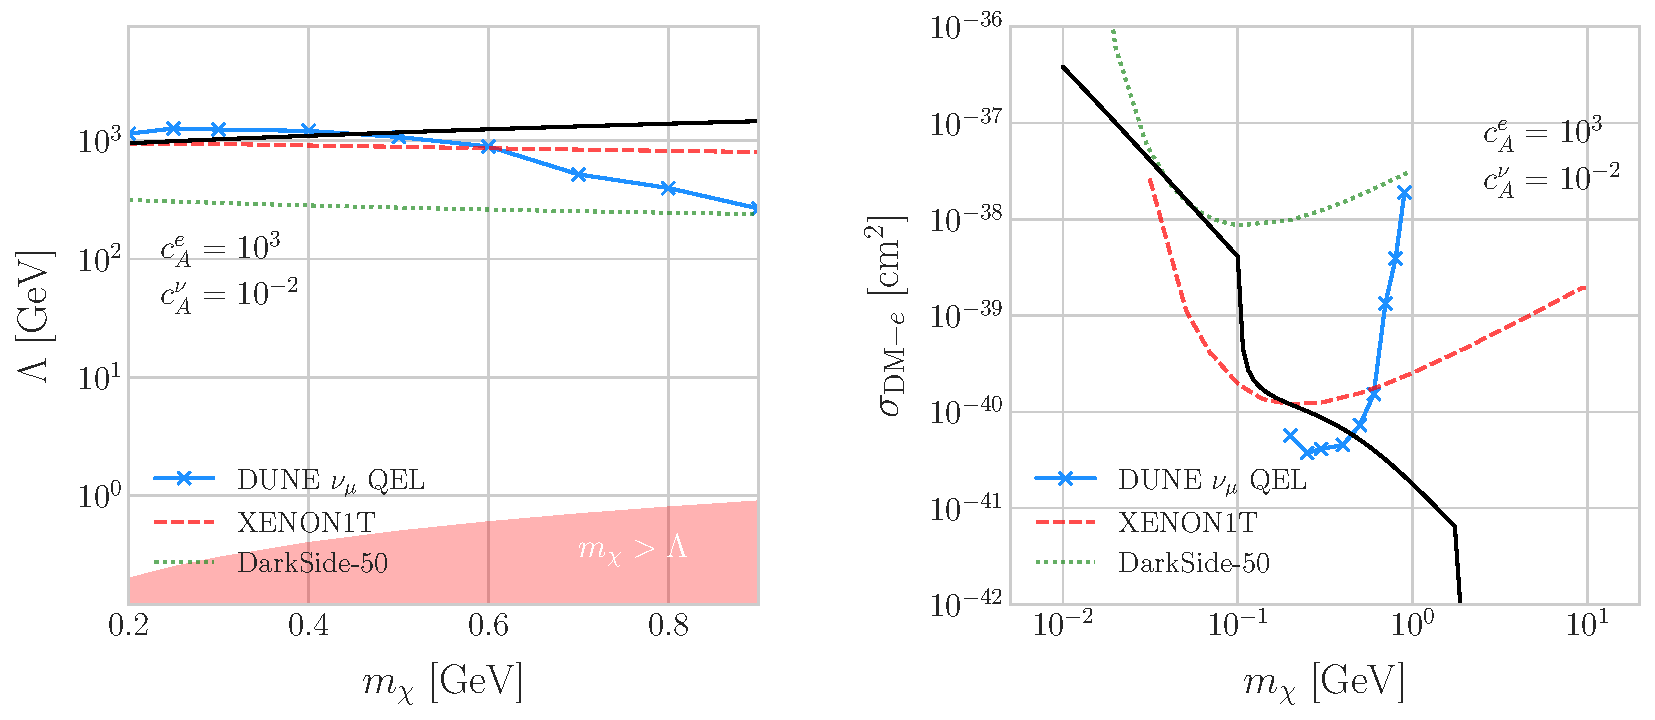
\includegraphics[width=1\linewidth]{Images/DM_Analysis/eft_bounds.pdf}
	\caption[Projected 90\% confidence level sensitivity of DUNE (400 kT yr) to the scale $\Lambda$ of an EFT containing only leptophilic DM axial-axial interactions.]{Left panel: Projected 90\% confidence level sensitivity of DUNE (400 kT yr) to the scale $\Lambda$ of an EFT containing only leptophilic DM axial-axial interactions (blue line), for the coupling values $c_{A}^{e} = 10^{3}$ and $c_{A}^{\nu} = 10^{-2}$. The black line represents the values for which the correct relic density is achieved. Right panel: Excluded values of $c_{A}^{\ell}$ as a function of the DM mass, for a fixed value $c_{A}^{\nu} = 10^{-2}$. In both cases the corresponding limits from XENON1T \cite{XENON2019} (red), DarkSide-50 \cite{DarkSide2022} (green) and PandaX-II \cite{PandaX-II2021} (magenta) are also shown.}
	\label{fig:eft_bounds}
\end{figure}

As discussed before, in the low DM mass region QE interactions dominate. Moreover, if I focus on direct annihilation to neutrinos, the energy of the muon neutrino flux is known as it must be equal to the mass of the DM particle, $E_{\nu} = m_{\chi}$. That way, now I do not need to use Eq. (\ref{6.6}) in order to estimate the momentum transfer to the remnant nucleus, I can simply take:
\begin{equation}\label{7.6}
	\vec{p}_{N} = \hat{p}_{\nu} m_{\chi} - \vec{p}_{\mu} - \vec{p}_{p}.
\end{equation}

To estimate the signal efficiency and background rejection for this case I used again the MLP classifier from \texttt{scikit-learn}, using the same specifications as before. The only difference now is that I add also the reconstructed neutrino energy as one of the features to train the classifier with, because the characteristic monoenergetic flux for each $m_{\chi}$ value will help to distinguish between signal and background events.

In this case, for masses below $\sim 500 \ \mathrm{MeV}$ I obtain a signal efficiency close to unity while keeping a background rejection of $99.9\%$. For bigger values of the mass, the signal efficiency drops significantly if I require to keep the background acceptance under $0.01\%$. However, because this kind of search is dominated by the background, sacrificing the signal acceptance to keep the background rejection to a minimum enhances the reach of the analysis. This way, for DM masses of the order of $m_{\chi} \sim 1 \ \mathrm{GeV}$ I end up with efficiencies as low as $1\%$.

Now, estimating the number of background events using Eq. (\ref{6.12}) one can go on and apply Eqs. (\ref{4.5}) and (\ref{4.6}) together with Eq. (\ref{7.3}) to derive the sensitivity of DUNE to this kind of model. Fig. \ref{fig:eft_bounds} (left panel) shows the potential reach of DUNE to constrain the EFT scale $\Lambda$ this model containing only leptophilic DM axial-axial interactions (blue line), for a choice of couplings $c_{A}^{e} = 10^{3}$ and $c_{A}^{\nu} = 10^{-2}$. I also included the current limits on the DM-electron scattering cross section from XENON1T \cite{XENON2019} (dashed red line), DarkSide-50 \cite{DarkSide2022} (dotted green line) and PandaX-II \cite{PandaX-II2021} (dash-dotted magenta line), reworked with Eq. (\ref{7.3}) to show their implications for the EFT scale. The values of $\Lambda$ for which the correct DM relic density value is achieved for each mass are also shown (black line). This tells us that, for that specific choice of couplings, DUNE would be sensitive to DM configurations allowed by the relic density constraint up to a mass of $m_{\chi} \sim 400 \ \mathrm{MeV}$.

In Fig. \ref{fig:eft_bounds} (right panel) I show similar limits for the excluded values of $c_{A}^{\ell}$ as a function of the DM mass, for a fixed $c_{A}^{\nu}=10^{-2}$. I do not show the limits for other values of $c_{A}^{\nu}$, as this parameter has little effect on the phenomenology at hand. From this view one can see that DUNE would be able to offer complementary information to the low energy DM-electron interaction searches performed by direct detection experiments, in a slightly higher mass range.

With the present example, although it focuses on a very specific realisation of the DM interactions, I show the potential of DUNE to constrain exotic DM scenarios. Thanks to its low backgrounds and superb angular resolution DUNE will be able to help with the systematic searches for dark sectors physics.

\section{Systematic uncertainties}
\label{sec:dm_analysis_systematics}

The estimation of the DM cross sections using neutrinos from WIMP annihilations inside the Sun is affected by systematic uncertainties from different sources. Surely, the atmospheric background estimation is also affected by systematic uncertainties. There are uncertainties common to both types of events, as well as others specific to each. In this section, I try to provide a comprehensive summary of the main sources of uncertainty for this analysis, which should be taken into account in any future extensions of the same.

\begin{table}[t]
	\caption[Systematic uncertainties for the solar WIMP signal events.]{Systematic uncertainties for the solar WIMP signal events. Table adapted from Ref. \cite{Principato2021}.}
	\begin{center}
		\begin{small}
			\begin{tabular}{c|c}
				Systematic                         & Value \\[2mm] \hline
				\rule{0pt}{1.1\normalbaselineskip}Form factor                      & Does not apply to SD \cite{Wikstroem2009} \\[2mm]
				Solar model                      & $3\%$ \cite{Wikstroem2009} \\[2mm]
				Local DM density                 & Not relevant for relative interpretations \cite{Wikstroem2009,Super-Kamiokande2015} \\[2mm]
				Dynamics of solar system         & Negligible \cite{Rott2011} \\[2mm]
				Velocity distributions           & $20\%$ at $20~\mathrm{GeV}$ \cite{Wikstroem2009,Super-Kamiokande2015} \\[2mm] \hline
				\rule{0pt}{1.1\normalbaselineskip}Oscillation parameters           & $8\%$ for $\tau^{+}\tau^{-}$, $5\%$ for $b\bar{b}$ \cite{Boliev2013} \\[2mm]
				Neutrino interactions in the Sun & $10\%$ \\[2mm]
				Matter effects in the Earth      & $10\%$ 
			\end{tabular}
		\end{small}
	\end{center}
	\label{tab:solar_dm_signal_uncertainties}
\end{table}

\subsection{Systematic uncertainties in the solar WIMP signal}

The systematic uncertainties affecting the solar WIMP neutrino signal can be divided in two categories. On the one hand, we have those affecting the solar WIMP annihilation rate. On the other hand, there are the ones which modify the neutrino flux resulting from the annihilations reaching our detector.

\begin{itemize}
	\item \textbf{Uncertainties on the annihilation rate}. These include the astrophysical effects that affect the normalisation of the solar DM neutrino flux. The main contributions are the solar model choice, the form factor uncertainties (only for SI searches), the gravitational effect of other planets, the local DM density (not relevant for relative comparisons, as it affects direct detection experiments in the same way), and the DM halo and dispersion velocities.
	\item \textbf{Uncertainties on the neutrino flux}. These are related to the oscillation effects, as well as the absorption and regeneration of neutrinos in the Sun. Matter effects inside the Earth also affect the neutrino flux the measured at the detectors.
\end{itemize}

Table \ref{tab:solar_dm_signal_uncertainties} summarises the contributions of the different sources of uncertainty for the signal events. These are the signal systematic uncertainties that have been taken into account in previous solar DM searches with neutrinos \cite{Boliev2013,Super-Kamiokande2015,Principato2021}.

\begin{table}[t]
	\caption[Systematic uncertainties for the solar WIMP atmospheric background events.]{Systematic uncertainties for the solar WIMP atmospheric background events. Table adapted from Ref. \cite{Super-Kamiokande2017}.}
	\begin{center}
		\begin{small}
			\begin{tabular}{c|c}
				Systematic                                            & Value \\[2mm] \hline
				\rule{0pt}{1.1\normalbaselineskip}Flux normalisation                                    & $25-7\%$ for $0.1 < E_{\nu} \leq 1~\mathrm{GeV}$ (linear in $\mathrm{log} ~ E_{\nu}$)\\[1mm] & $7\%$ up to $10~\mathrm{GeV}$ \\[2mm]
				$(\nu_{\mu}+\bar{\nu}_{\mu})/(\nu_{e}+\bar{\nu}_{e})$ & $2\%$ for $E_{\nu} \leq 1~\mathrm{GeV}$ \\[1mm] & $3\%$ for $1 < E_{\nu} \leq 10~\mathrm{GeV}$ \\[2mm]
				$\bar{\nu}_{\mu}/\nu_{\mu}$                           & $2\%$ for $E_{\nu} \leq 1~\mathrm{GeV}$ \\[1mm] & $6\%$ for $1 < E_{\nu} \leq 10~\mathrm{GeV}$ \\[2mm]
				$\mathrm{K}/\pi$ ratio                                & $5\%$ $E_{\nu} \leq 100~\mathrm{GeV}$
			\end{tabular}
		\end{small}
	\end{center}
	\label{tab:solar_dm_background_uncertainties}
\end{table}

\subsection{Systematic uncertainties in the atmospheric background}

For the atmospheric background events, one needs to take into account the systematic uncertainties affecting the atmospheric $\nu_{\mu}$ flux. These have been extensively studied in the context of atmospheric neutrino oscillation measurements. Among these, the energy-dependent flux normalisation uncertainty is the in the low energy regime. Other important contributions to the uncertainty come from the ratios between the muon to electron neutrino and the muon to anti-muon neutrino components of the flux. Additional uncertainty is introduced by the errors in the pion and kaon production rates calculated for the hadronic interactions of cosmic rays in the atmosphere \cite{Honda2006}.

Table \ref{tab:solar_dm_background_uncertainties} shows a summary of the leading contributions to the uncertainty on the atmospheric muon neutrino flux, in the energy range relevant for this analysis.

\subsection{Common systematic uncertainties}

Finally, there are sources of uncertainty common to both signal and backgrounds. These have two different origins:

\begin{itemize}
	\item \textbf{Uncertainties on the neutrino cross section}. These are introduced by the modelling of the neutrino-nucleus interactions. In the context of the solar WIMP analysis, these have been estimated to be $10\%$ for DM masses around $10~\mathrm{GeV}$ \cite{Boliev2013}.
	\item \textbf{Uncertainties related to the detector}. They affect the measurement of the neutrino interaction and the final state particles produced. The main detector uncertainties relevant to this analysis are those of the energy and angular resolutions of the DUNE FD. Other effects, like the timing and triggering efficiencies, will also contribute to the uncertainties. The particular values these will take for this analysis need to be worked out in the context of DUNE.
\end{itemize}